%% The main file. It contains definitions of basic parameters and includes all other parts.

%% Settings for single-side (simplex) printing
% Margins: left 40mm, right 25mm, top and bottom 25mm
% (but beware, LaTeX adds 1in implicitly)
\documentclass[12pt,a4paper]{report}
\setlength\textwidth{145mm}
\setlength\textheight{247mm}
\setlength\oddsidemargin{15mm}
\setlength\evensidemargin{15mm}
\setlength\topmargin{0mm}
\setlength\headsep{0mm}
\setlength\headheight{0mm}
% \openright makes the following text appear on a right-hand page
\let\openright=\clearpage

%\renewcommand{\baselinestretch}{1.5} 

%% Settings for two-sided (duplex) printing
% \documentclass[12pt,a4paper,twoside,openright]{report}
% \setlength\textwidth{145mm}
% \setlength\textheight{247mm}
% \setlength\oddsidemargin{14.2mm}
% \setlength\evensidemargin{0mm}
% \setlength\topmargin{0mm}
% \setlength\headsep{0mm}
% \setlength\headheight{0mm}
% \let\openright=\cleardoublepage

%% Character encoding: usually latin2, cp1250 or utf8:
\usepackage[utf8]{inputenc}

%% Further useful packages (included in most LaTeX distributions)
\usepackage{amsmath}        % extensions for typesetting of math
\usepackage{amsfonts}       % math fonts
\usepackage{amsthm}         % theorems, definitions, etc.
\usepackage{bbding}         % various symbols (squares, asterisks, scissors, ...)
\usepackage{bm}             % boldface symbols (\bm)
\usepackage{graphicx}       % embedding of pictures
\usepackage{fancyvrb}       % improved verbatim environment
%\usepackage{natbib}         % citation style AUTHOR (YEAR), or AUTHOR [NUMBER]
\usepackage[round]{natbib}
\usepackage[nottoc]{tocbibind} % makes sure that bibliography and the lists
			    % of figures/tables are included in the table
			    % of contents
\usepackage{dcolumn}        % improved alignment of table columns
\usepackage{booktabs}       % improved horizontal lines in tables
\usepackage{paralist}       % improved enumerate and itemize
\usepackage[usenames]{xcolor}  % typesetting in color

\usepackage{multirow}
%\usepackage{obo-cite}

\usepackage{listings}
%\usepackage{breakcites}

\usepackage{threeparttable}

%%% Basic information on the thesis

% Thesis title in English (exactly as in the formal assignment)
\def\ThesisTitle{Automatic Error Correction of Machine Translation Output}

% Author of the thesis
\def\ThesisAuthor{Dušan Variš}

% Year when the thesis is submitted
\def\YearSubmitted{2016}

% Name of the department or institute, where the work was officially assigned
% (according to the Organizational Structure of MFF UK in English,
% or a full name of a department outside MFF)
\def\Department{Institute of Formal and Applied Linguistics}

% Is it a department (katedra), or an institute (ústav)?
\def\DeptType{Institute}

% Thesis supervisor: name, surname and titles
\def\Supervisor{RNDr. Ondřej Bojar, Ph.D.}

% Supervisor's department (again according to Organizational structure of MFF)
\def\SupervisorsDepartment{Institute of Formal and Applied Linguistics}

% Study programme and specialization
\def\StudyProgramme{Master of Computer Science}
\def\StudyBranch{Mathematical Linguistics}

% An optional dedication: you can thank whomever you wish (your supervisor,
% consultant, a person who lent the software, etc.)
\def\Dedication{%
I would like to thank my supervisor, RNDr. Ond\v{r}ej Bojar, Ph.D., for valuable
advice and support during writing this thesis. I would also like to thank
Mat\v{e}j Trojan for helping me with the evaluation of Czech MLFix output. Finally,
I would like to thank Ladislav Valkovi\v{c}, Ph.D. and Radek S\'{i}le\v{s} for
helping me with evaluating German MLFix output and providing me information about the language.

This thesis is dedicated to them.
}

% Abstract (recommended length around 80-200 words; this is not a copy of your thesis assignment!)
\def\Abstract{%
We present MLFix, an automatic statistical post-editing system, which is a spiritual successor of the rule-based
Depfix system. The aim of this is to investigate the possible approaches to automatic identification
of the most common morphological errors produced by the state-of-the-art machine translation systems and
to train a sufficient statistical models built on the acquired knowledge. The system was mainly developed on the English-to-Czech
machine translation output, however, the aim was to generalize the post-editing process so it can be
applied to other language pairs. For this reason, we also present the results of experiments done on the English-German
language pair.
}

% 3 to 5 keywords (recommended), each enclosed in curly braces
\def\Keywords{%
{automatic post-editing,} {machine translation,} {supervised machine\newline
learning,} {natural language processing,} {Treex}
}

%% The hyperref package for clickable links in PDF and also for storing
%% metadata to PDF (including the table of contents).
\usepackage[pdftex,unicode]{hyperref}   % Must follow all other packages
\hypersetup{breaklinks=true}
\hypersetup{pdftitle={\ThesisTitle}}
\hypersetup{pdfauthor={\ThesisAuthor}}
\hypersetup{pdfkeywords=\Keywords}
\hypersetup{urlcolor=blue}


%%%% Custom Definitions %%%

\newcommand{\fixme}[1]{\textcolor{red}{FIXME: (#1)}} % macro for fixme entries
\newcommand{\todo}[1]{\textcolor{blue}{TODO: (#1)}} % macro for todo entries

\def\samp#1{``\textit{#1}''}
\def\pojem#1{\textit{#1}}
\def\code#1{\texttt{#1}}


\def\Tref#1{Table~\ref{#1}}
\def\Fref#1{Figure~\ref{#1}}
\def\Eref#1{Example~\ref{#1}}
\def\Sref#1{Section~\ref{#1}}
\def\Cref#1{Chapter~\ref{#1}}
\def\Mref#1{Formula~\ref{#1}}
\def\equo#1{``#1''}
\def\notion#1{{\emph{#1}}}
\def\perscite#1{\newcite{#1}}
\def\parcite#1{\cite{#1}}
\def\footurl#1{\footnote{\url{#1}}}
\def\hash{\#}
\def\tilda{\~{}}


%%%%%%%%%%%%%%%%%%%%%%%%%%%

% Definitions of macros (see description inside)
%%% This file contains definitions of various useful macros and environments %%%
%%% Please add more macros here instead of cluttering other files with them. %%%

%%% Minor tweaks of style

% These macros employ a little dirty trick to convince LaTeX to typeset
% chapter headings sanely, without lots of empty space above them.
% Feel free to ignore.
\makeatletter
\def\@makechapterhead#1{
  {\parindent \z@ \raggedright \normalfont
   \Huge\bfseries \thechapter. #1
   \par\nobreak
   \vskip 20\p@
}}
\def\@makeschapterhead#1{
  {\parindent \z@ \raggedright \normalfont
   \Huge\bfseries #1
   \par\nobreak
   \vskip 20\p@
}}
\makeatother

% This macro defines a chapter, which is not numbered, but is included
% in the table of contents.
\def\chapwithtoc#1{
\chapter*{#1}
\addcontentsline{toc}{chapter}{#1}
}

% Draw black "slugs" whenever a line overflows, so that we can spot it easily.
\overfullrule=1mm

%%% Macros for definitions, theorems, claims, examples, ... (requires amsthm package)

\theoremstyle{plain}
\newtheorem{thm}{Theorem}
\newtheorem{lemma}[thm]{Lemma}
\newtheorem{claim}[thm]{Claim}

\theoremstyle{plain}
\newtheorem{defn}{Definition}

\theoremstyle{remark}
\newtheorem*{cor}{Corollary}
\newtheorem*{rem}{Remark}
\newtheorem*{example}{Example}

%%% An environment for proofs

%%% FIXME %%% \newenvironment{proof}{
%%% FIXME %%%   \par\medskip\noindent
%%% FIXME %%%   \textit{Proof}.
%%% FIXME %%% }{
%%% FIXME %%% \newline
%%% FIXME %%% \rightline{$\square$}  % or \SquareCastShadowBottomRight from bbding package
%%% FIXME %%% }

%%% An environment for typesetting of program code and input/output
%%% of programs. (Requires the fancyvrb package -- fancy verbatim.)

\DefineVerbatimEnvironment{code}{Verbatim}{fontsize=\small, frame=single}

%%% The field of all real and natural numbers
\newcommand{\R}{\mathbb{R}}
\newcommand{\N}{\mathbb{N}}

%%% Useful operators for statistics and probability
\DeclareMathOperator{\pr}{\textsf{P}}
\DeclareMathOperator{\E}{\textsf{E}\,}
\DeclareMathOperator{\var}{\textrm{var}}
\DeclareMathOperator{\sd}{\textrm{sd}}

%%% Transposition of a vector/matrix
\newcommand{\T}[1]{#1^\top}

%%% Various math goodies
\newcommand{\goto}{\rightarrow}
\newcommand{\gotop}{\stackrel{P}{\longrightarrow}}
\newcommand{\maon}[1]{o(n^{#1})}
\newcommand{\abs}[1]{\left|{#1}\right|}
\newcommand{\dint}{\int_0^\tau\!\!\int_0^\tau}
\newcommand{\isqr}[1]{\frac{1}{\sqrt{#1}}}

%%% Various table goodies
\newcommand{\pulrad}[1]{\raisebox{1.5ex}[0pt]{#1}}
\newcommand{\mc}[1]{\multicolumn{1}{c}{#1}}

%%% Example environment
\newcounter{excounter}
    \newenvironment{myexample}[0]{%
    \bigskip\noindent%
    \refstepcounter{excounter}%
    \newline%
}
{%
    \begin{center}%
    \textsc{\theexcounter}%
    \end{center}%
    \par\bigskip%
}
\numberwithin{excounter}{chapter}


% Title page and various mandatory informational pages
\begin{document}
%%% Title page of the thesis and other mandatory pages

%%% Title page of the thesis

\pagestyle{empty}
\hypersetup{pageanchor=false}
\begin{center}

\centerline{\mbox{
\includegraphics[width=166mm]{img/logo.pdf}}}

\vspace{-8mm}
\vfill

{\bf\Large MASTER THESIS}

\vfill

{\LARGE\ThesisAuthor}

\vspace{15mm}

\begin{center}
\LARGE\bfseries\ThesisTitle
\end{center}
%{\LARGE\bfseries\ThesisTitle}

\vfill

\Department

\vfill

\begin{tabular}{rl}

Supervisor of the master thesis: & \Supervisor \\
\noalign{\vspace{2mm}}
Study programme: & \StudyProgramme \\
\noalign{\vspace{2mm}}
Study branch: & \StudyBranch \\
\end{tabular}

\vfill

% Zde doplňte rok
Prague \YearSubmitted

\end{center}

\newpage

%%% Here should be a bound sheet included -- a signed copy of the "master
%%% thesis assignment". This assignment is NOT a part of the electronic
%%% version of the thesis. DO NOT SCAN.

%%% A page with a solemn declaration to the master thesis

\openright
\hypersetup{pageanchor=true}
\pagestyle{plain}
\pagenumbering{roman}
\vglue 0pt plus 1fill

\noindent
I declare that I carried out this master thesis independently, and only with the cited
sources, literature and other professional sources.

\medskip\noindent
I understand that my work relates to the rights and obligations under the Act No.~121/2000 Sb.,
the Copyright Act, as amended, in particular the fact that the Charles
University has the right to conclude a license agreement on the use of this
work as a school work pursuant to Section 60 subsection 1 of the Copyright Act.

\vspace{10mm}

\hbox{\hbox to 0.5\hsize{%
In ........ date ............	% FIXME!
\hss}\hbox to 0.5\hsize{%
signature of the author
\hss}}

\vspace{20mm}
\newpage

%%% Mandatory information page of the thesis

\openright

\vbox to 0.5\vsize{
\setlength\parindent{0mm}
\setlength\parskip{5mm}

Title:
\ThesisTitle

Author:
\ThesisAuthor

\DeptType:
\Department

Supervisor:
\Supervisor, \SupervisorsDepartment

Abstract:
\Abstract

Keywords:
\Keywords

\vss}

\newpage

%%% Dedication

\openright

\noindent
\Dedication

\newpage

\openright
\pagestyle{plain}
\pagenumbering{arabic}
\setcounter{page}{1}


%%% A page with automatically generated table of contents of the master thesis

\setcounter{page}{1}
\tableofcontents

%%% Each chapter is kept in a separate file
\chapter{Introduction}
%\chapter*{Introduction}
%\addcontentsline{toc}{chapter}{Introduction}

In this thesis, we are presenting a statistical post-editing tool MLFix
based on its rule-based predecessor Depfix \citep{depfix:2014}.
We aim to use statistical machine learning methods to generalize a subset of Depfix rules
with focus on creating fairly language-independent automatic post-editing (APE) tool.
Our main goal is to find a reasonable tradeoff between the amount
of linguistic knowledge gathered from the input data and the dependence
on the language-specific third-party analysis tools, to specify the
machine learning (ML) task which our APE component should accomplish and to train
a sufficient ML model for correcting the machine translation (MT) output.
The system was developed using English-Czech language pair, however, we also present
a preliminary results we gathered from English-German language pair experiments.

\section{Task Motivation}

Even though the current state-of-the-art MT systems have been gradually improving in the
past few decades, they are still not perfect. Currently the most popular statistical machine
translation (SMT) systems can be fairly effective even without any or a little initial
linguistic knowledge about the concerned language pair given they have access to sufficient
amount of parallel data. However, when translating into the morphologically rich languages,
the data sparsity increases rapidly and such systems quickly begin to introduce grammatical
errors into the translated sentences and worsen the overall fluency of the translation.

Still, these systems can be of help to the human translators since it is usually less costly
to have even partially incorrect translations provided by the SMT system and have
human translator correct them then to translate the source text manually.
Human post-editors can however still be a quite costly so naturally there have been
attemts to automate this process with automatic post-editing tools.

\section{Related Work}

Up to this date there have been various approaches to the task of automatic
error correction of the machine translation output, each with a different level of success.

The very first attempts in the field of automatic post-editing \citep{simard2007rule}
focused on applying phrase-based statistical machine translation (PB-SMT)
system on the output of the rule-base machine translation. The system was trained on a monolingual
bitextual data containing the MT output as a source sentence and a reference translation as
the target sentence. This phrase-based automatic post-editor (PB-APE) helped to significantly improve
the performance of the rule-based MT system in question.
There were also attempts to apply the post-editing component
on a phrase-based translation system but the combined system performed slightly worse in comparison
with the standalone SMT system.

Further experiments with PB-SMT $+$ PB-APE \citep{bechara:2011} were done
on English-French and French-English translation, where significant improvements were reported
for the latter translation direction. They improved the design suggested by Simard et al. by
creating the purely statistical pipeline. The PB-APE was then expanded by adding additional
context information about the source sentence to SMT-generated output (used as an input for
the PB-APE) reporting further improvement in performance. However, the presented system failed to
improve the MT output in the opposite translation direction (English-French).

These previous attempts can be considered purely statistical since only a little ammount of linguistic
knowledge about the concerned languages was used during developement. To gain further insight into
the task of automatic post-editing, more thorough analysis of the most frequent errors made by the current
SMT systems was performed by \citet{bechara:master} and later by \citet{biblio:RoAutomaticpostediting2013}, the former
for English-French and the latter for English-Czech.

The error analysis was later used during developement of the rule-based APE Depfix \citep{depfix:2014},
which was designed to correct the errors made by the English-Czech SMT systems.
The system uses a set of finely hand crafterd rules that aim at identifying
and correcting morphological errors such as incorrect agreement or valency, which are
often encountered during English-Czech machine translation. It does not focus on a lexical errors
although some minor corrections, e.g. insertion of missing reflexive verbs, are made. The system
succeeded to improve output of various MT systems and was deployed as a stable part of the
Chimera \citep{biblio:BoRoChimera2013} MT system.

The idea behind Depfix system seems promising, however, due to its rule-based nature, it is difficult
to apply the APE on different language pair since it would required costly modifications to the
existing set of rules. One of the goals of this thesis is to try and replace the rule-based blocks
by a statistical ones so they applied to the different target language MT output more easily simply
by training an appropriate statistical model.

%"Better Evaluation for Grammatical Error Correction" Dahlmeier
% napsat az do model tuningu ???
% Correction model for non-MT generated errors (classification)
% Important -> balancing training data

\section{Thesis Structure}
%strucny popis depfixu? popis castych chyb ???

%odkazy
In~Chapter~\ref{chap:system_descr}, we describe MLFix data processing
pipeline and introduce all the tools we use.
In~Chapter~\ref{chap:data}, we take a look at all datasets which we used during our system
developement and analyze their usefulness for our system.
In~Chapter~\ref{chap:task_descr}, we define the post-editing task, go through
various modifications of the task we considered and explain our though
process with support of the analysis of the available data.
In~Chapter~\ref{chap:tuning}, we describe the process of the developement
the statistical models for the MLFix post-editing component and present
a preliminary results of the evaluation of the trained models.
In~Chapter~\ref{chap:eval}, we evaluate the performance of the whole MLFix system
and analyze the level of contribution to the resulting performance
of each individual statistical compocomponent.
In~Chapter~\ref{chap:german}, we briefly describe our modifications to English-Czech pipeline
when used on English-German language pair, then summarize the differences
in the training data and model training between the two language pairs. The Chapter concludes with evaluation of English-German pipeline.
%In chapter 8, we present performance results of the modified English-German
%pipeline.
We conclude the thesis in Chapter 9.

We include a full English-Czech and English-German Treex scenario in Attachment~\ref{attach:scen}.

\fixme{Dodatek k attachmentum}



\chapter{System description}
\label{chap:system_descr}

In this chapter we describe the main components
of MLFix system and take a closer look at the suggested processing pipeline.
We focus on English-Czech pipeline, however, we also describe modifications
needed to apply MLFix for other language pairs.

Full examples of currently deployed Treex scenarios (English-Czech and English-German)
are included in Attachment~\ref{attach:scen}.

%The main idea of MLFix system is to analyze the provided input data providing
%a set of input features 

\section{Processing pipeline}

MLFix is, similarly to its predecessor, almost entirely implemented in the
Treex \citep{Popel:2010:TMN:1884371.1884406}\footurl{http://ufal.mff.cuni.cz/treex}
framework (formerly knownas TectoMT).
The framework was originally created as English-Czech hybrid translation system, combining
rule-based modules with statistical models and using deep semantic language representation
for the sentence translation. However, due to its modularity, it is
now used for various tasks of natural language processing (NLP) across different
languages. The framework was built to support a methodology of the theory of Functional Generative Description \citep{Sgall1967}
and was adapted to support sentence representation in Prague Dependency Treebank \citep{pdt20:2006}.
Mainly, it supports the representation of sentences on different layers of abstaction defined in FGD: morphological layer,
analytical layer and a tectogrammatical layer.\footnote{Usually referred to as m-layer, a-layer and t-layer where prefixes m-, a- and t- are also used to refer to the objects on the corresponding layer of abstraction.}
Because the tools currently available for tectogrammatical layer analysis are available for
a limited set of languages (mainly Czech and English, a developement of others is in progress),
we decided to use only the a-layer (surface syntax) for data representation.

\subsection{M-Layer analysis}

MLFix analysis pipeline is derived from an existing Depfix pipeline
with a several modifications to make it easier to apply to different
target languages. Input data (source sentence + MT output aligned on a sentence level,
or additionaly reference sentences for extracting the training data)
are first read in parallel and stored into Treex internal representation.
Both source side and MT side are tokenized by a rule-based tokenizer, each token is then
represented by a separate m-node.

Next, a lemmatization and part-of-speech (POS) tagging is performed on each m-node.
For both English and Czech, we use MorphoDiTa \citep{strakova14:morphodita}\footurl{http://ufal.mff.cuni.cz/morphodita}
tool for morphological analysis and tagging. MorphoDiTa is also used for Czech lemmatization.
For English lemmatization, we use a rule-based block implemented in Treex.
It is important to provide a POS tagger for the target language that supports
relatively fine-grained morphological tags because our goal is to correct morphological
errors represented mainly through these tags.
It was reported by Rosa\fixme{znovu citovat diplomku?} that tagger produces significantly more
errors in morphological analysis of Czech SMT outputs. In Depfix, this is covered
by a rule-based block that identifies these errors and changes the incorrect POS tag without
changing the surface form. We decided to omit this block and leave the issue to our statistical
component.

Last step we do in the scope of the m-layer analysis is a transformation of the POS tags into
a more general representation. Optionally we can apply a named-entity recognition
tool if one is available but it isn't mandatory. For English, we use the Stanford
Named Entity Recognizer (NER) \citep{Finkel:2005:INI:1219840.1219885}\footurl{http://nlp.stanford.edu/software/CRF-NER.shtml},
for Czech, we use a simple rule-based NER. 

\subsection{Interset}

Since there are usually different tagsets used across individual languages,
often engineered for purposes of that specific language and with no standardized
tag representation,
we would be forced to modify our existing pipeline to some extent everytime
a new language would be introduced.
Therefore we decided to use Interset \citep{biblio:ZeReusableTagset2008}\footurl{https://ufal.mff.cuni.cz/interset}, an interlingua-based
representation of POS tags from various tagsets. To be able to use this
representation to represent tags from a given tagset, a decoding/encoding
module is required. However, the support for various tagsets spanning
through different languages started growing lately mainly due to Universal Dependencies \citep{universal-dep:2016}\footurl{universaldependencies.org} project.

After the transformation, in following steps of the analysis, a choice
of a specific tagset becomes transparent because MLFix blocks only
have to deal with one well-defined set of features.

\subsection{Word alignment}

In the next step, we create a word-level alignment between each sentence pair
using GIZA++ \citep{och:ney:2000}. We make one-to-one word alignment where possible
using an intersection symmetrization. This step helps us later with feature extraction
and with further processing of the target sentence.

In the process of training data extraction, we also create a simple alignment between
the MT sentence and the reference sentence exploiting forms, lemmas and tags
of the m-nodes. The alignment between the source sentence and the MT ouptut is then also
projected to the reference sentence.

\subsection{A-Layer analysis}

After the m-layer analysis and the word alignment, we perform a dependency parsing.
For English, we use Maximum spanning tree (MST) parser \citep{mcdonald:pereira:ribarov:hajic:2005}\footurl{http://sourceforge.net/projects/mstparser}
implemented in Treex framework. For SMT output, even though there might
be an existing dependency parser available for the target language, it is usually
trained on data that do not contain errors. Therefore, it has usually significantly
lower performance when applied on the SMT output. Still research on Depfix have shown
that a knowledge of the dependency structure of the SMT output can provide additional
valuable information for identifying grammatical errors\footnote{Actually, in the case of Depfix
, the information about the dependency structure is crucial for most of the fixing components
because e.g. a parent-child relationship is examined almost everytime.}, thus improving
the post-editor's performance.

For the time being we have decided to build the dependency structures of the SMT output simply
by projecting the dependency structure of the source sentence onto the target side
using the word alignment we extracted in the preceeding step. The resulting structure
is likely to contain errors, but should be at least consistent thoughout our data.
To compensate for the lower accuracy of the extracted dependency structure we perform
a dependency parsing of the reference sentences during training, if a proper parser
is available. For this purposes, we use the MST Parser for the Czech language as well.
We expect that the combination of dependency parser for the reference sentences and
a right choice of constraints applied when extracting training instances we should
avoid polluting our training data with instances containing misleading context information
due to an incorrect structure of the SMT dependency tree.

For Czech SMT output, an implementation of the MST parser adapted for the SMT output
is already available \citep{biblio:RoDuUsingParallel2012}, however, so far we haven't done any experiments
to determine whether the dependency structures provided by the adapted parser (which
should be more accurate) influence the final performance of our system.

%\subsection{Training pipeline}

%We also do preprocessing of data we use for training our statistical component.
%The pipeline is similar to the processing pipeline with addition of processing
%the reference sentences. The reference sentences are processed in a same way
%as the MT output, however they are not analyzed on the a-layer, only a simple
%lemma based word alignment with the MT output is made.

\section{Statistical component}

After data preprocessing, we extract all available features and
apply a trained statistical model. The features are extracted separetely for each node and passed
to a model. The model needs to accomplish these two goals:
\begin{enumerate}
    \item identify candidates with incorrect morphology,
    \item fix incorrect morphological features.
\end{enumerate}
Of course, these two steps can be split between multiple separate components (and models).
We describe the post-editing process in more detail later in chapter~\ref{chap:tuning}.

We decided to use Scikit-Learn \citep{scikit-learn}\footurl{biblio:RoDuUsingParallel2012} toolkit to train and execute our models since
it has easy-to-use and quite uniform interface, which allows us to try out different
machine learning (ML) methods simply by switching the model class. In Treex, we use a simple
wrapper to load and execute the trained Scikit-Learn model. If a support for a different ML implementation
is needed (e.g. VowpalWabbit\footurl{https://github.com/JohnLangford/vowpal\_wabbit/wiki}\footnote{At the time of writing this thesis, there is already
a limited support for VowpaWabbit.}), this wrapper can be easily modified to suit the requirements.

\section{Wordform generation}

After we have identified morphologically incorrect words and assigned
them a new morphological categories we need to generate a new surface form reflecting
the changes we have made.
This can be done either by rule-based component or with
help of another statistical model. 

For Czech, we have used a morphological generator build upon the morphology of \citet{HajicHAB2004}
that is already a part of Treex framework. For other languages,
when there was not another option available,
we have used Flect \citep{DBLP:conf/acl/DusekJ13}\footurl{https://ufal.mff.cuni.cz/flect}.
It is a language independent morphological generation tool also using Scikit-Learn
models. The tool learns morphological inflection patters form an annotated corpora and
should able to inflect even previously unseen words using lemma suffixes as features
and predicting a difference between a lemma and a surface form.

\section{Language independence}

From the previous description, we can notice that MLFix still depends on several
language specific tools. It is quite dependent on the capability of a source
language analysis (in our case English), because we do not only need a POS tagger but also a dependency
parser. However, we assume that the source sentences are usually grammatical correct
so it is much easier to provide required tools than their modified versions
targeted at the MT output.

We also require a specific decoder of the source and target POS tags into Interset feature
structures but Interset already covers large variety of the most widespread tagsets available
and its support is still growing.

Finaly, aside from a language specific post-editing models (which we do not expect
to be reusable across different languages) we require a module that regenerates
a correct wordform (either from the \samp{lemma+tag} or \samp{lemma+Interset features combination}).
A state-of-the-art tool might not be explicitly available for every language but if no
other option is provided we can use a statistical form generator, in our case Flect.

\chapter{Available data}

% dostupna data
% mnozstvi
% popis
% vyuziti

XXX TOTO ZREJME AZ DO POPISU SYSTEMU

In this chapter we are going to describe the format of the input data, that
our system require for training and present all the available datasets.
The differences between the suggested data can seem minor but they can
have impact on the overall performance of the system.

To train our system, we require sentence-level aligned set of source sentences,
MT output and a reference sentences
%TODO: footnote - reference in this thesis as a triparallel data
. The reference sentences can be either
a classic reference translation of the source text or a result of a human
post-editation of the MT output, they are however required because they
provide use with the possible corrections of the MT output.
Naturally, the closer the MT output is
to the reference translation, the easier it should be for our system
to extract valuable learning instances form the sentences. We also
considered using only pair of sentence aligned pair of MT translated
sentences and the reference sentences however, this way the trained
model will lose some of the useful features which can be extracted from
the triparallel data.

XXX

In this chapter we are going to take a closer look at the available
sources of data and describe how they contributed to our research.

We came across a various sources of training data with various level
of usefulness and usually of a smaller volume. Some of the sources
are:
\begin{itemize}
\item Khan's school human
post-edits of manually translated (EN$\rightarrow$CS) subtitles,
\item the Autodesk
triparallel data\footurl{https://autodesk.app.box.com/Autodesk-PostEditing},
\item log files of human post-editing done by Lingea for the
HimL\footurl{http://www.himl.eu/} project test dataset,

% uvest QT21?
%\item data from the QT21 project\footurl{http://www.qt21.eu/deliverables/annotations/},

%TODO: wmt - odkaz, footnote?
\item results from the previous workshops on machine translation (WMTs).
\end{itemize}

In the following sections, we will describe in more detail each of the datasets.

\subsection{Khan's school}

The data provided by Khan's school consist of en-cs subtitles,
where the Czech part (usually manually translated from English) was manually
edited. During the analysis of the dataset,
we've noticed that most of the time, the corrections were made
mostly on a lexical level which is only natural since the Czech sentences
were created by a human translator.
Therefore, we decided to avoid using this dataset for the time being or to
rather treat the corpus as a simple bilingual data.

\subsection{Autodesk}

Autodesk data consist of English sentences which were machine translated into
a set of target languages (cs, de, pl etc.) complemented with human post-editing
of MT output. These datasets are domain specific (mostly user documentations)
however, so they might not be very attractive to use with more general texts.
We weren't able to gather any information about the MT system that was used
to create the translated output. The biggest advantage of these data is
their larger volume when compared with other post-editing datasets so we
used them mainly for model developement and benchmarking of the used machine
learning methods.

\subsection{HimL-Lingea logs}

The data provided by Lingea were collected when official HimL test sets were
created. The data consist mainly of the public health related texts.
The original English sentences were first
machine-translated to HimL languages (Czech, German, Polish and Romanian)
and then post-edited by professional
translators using Lingea's post-editing tool. The datasets are probably the most
detailed one since they consist of complete logfiles
describing elementary actions taken by human post-editors (such as selecting
phrases in a translated sentence, looking up alternative translations
in a dictonary etc.).

When we examined the data more closely,
we noticed that it is rather difficult to determine which actions are
useful for our machine learning process. Also, we were little disapointed
when we found out that most of the time, the post-editors preferred to
rewrite the whole sentence "from scratch"\footnote{By that, we mean that the
translator usually preffered to write the whole corrected sentence, even though
only a several changes (both lexical and morphological), and delete the original.
This was also probably motivated by the need of reordering in the MT translated
sentence.} opposite to doing more atomic modifications to the provided MT output.

In the end, we decided to simply extract a triparallel data from these logs (the source
sentence + SMT output + result of the human post-editing). In the future,
we might consider to use other logged actions for model training.

\subsection{WMT datasets}

For the last decade, the workshop on machine translation (WMT) has aimed
to provide working grounds for many researchers in the field of machine
translation. It has been great source of the parallel data between English
on one side and various other languages on the other. Each year, the scope
of the workshop expands, including various new subtask related to machine translation,
such as several evaluation tasks and, more recently, automatic post-editing task.

The data available for the post-editing task usually contains a set of:
\begin{itemize}
    \item source English sentences,
    \item output of various MT systems, usually the ones that participate in the main
translation tasks,
    \item human post-edition of the mixed MT output from the participating MT systems.
    \fixme{je tohle pravda?}
\end{itemize}

These datasets gives us the opportunity to compare the performace of our post-editing
models when applied to the different systems. Even though the data available for the
WMT subtasks are from various domains (news, IT, biomedical), the domain of the post-editing
data is more limited, mainly to the news articles.

\subsection{Other sources}

The sources listed above (each one to a different degree, maybe except for the last one) can
be considered a knowledge base for examining the behaviour of a human post-editor as well
as training data for our system. We think that they might provide us
some interesting insight into the post-editor's thought process. On the other hand,
might also consider using some other sources since the sources mentioned above are quite
limited.

One possible way to face the data sparsity is to use available parallel corpora.
These corpora (containing only \notion{source sentences + reference translations})
can be expanded by translating the source sentences and thus creating a set of 
sentences which contain MT generated errors and should be fixed to resemble the 
reference translation. These data can be then used to train models for that
specific SMT system\footnote{Obviously, the post-editing model training data have to be
different from the parallel data used for the training of the SMT system, so
some
jackknife sampling should be used with limited training data.} or possibly for
another SMT systems.
This method can surely help to overcome the aforementioned data acquisition bottleneck
since there is generally much more parallel data then post-edited sentences. For
English-Czech language pair, the natural choice of the parallel corpus would be
CzEng~1.0\footurl{http://ufal.mff.cuni.cz/czeng} \cite{czeng10:lrec2012}.
We didn't use this approach in the scope of this thesis however, it might
be considered in our future work.
\todo{posledni vetu az do shrnuti?}

Of course, this aproach introduces some additional noise
related to the post-editing task. For example, we can get fluent MT output which
is just a variation on the reference translation (possibly thanks to the different
choice of wording etc.). It can be therefore hard to distinguish these fairly correct training
instances from the incorrect ones.

The basic summary of the available data is shown in the table \Tref{avail-data}.

\subsection{Monolingual data}

We also considered simply using bitext monolingual data (either \notion{MT output + post-edited sentences}
or \notion{MT output + reference translations}), however due to the nature of our processing
pipeline we would be much more limited when analyzing the training data. Also, as
mentioned by Rosa\cite{depfix:2014}, the additional information that can be
extracted from the source
sentences proved to be valuable in the practice.

%Even if we do not use this approach for the training of the final MLFix models,
%the volume of the data might help us with feature selection and preliminary model evaluation.

\begin{table*}[t]
\centering
\small

\begin{tabular}{lcccc}
\multirow{2}{*}{}  &  \multirow{2}{*}{\hash{} Sentences}  &  \multicolumn{3}{c}{\hash{} Tokens}  \\
&   & English & Czech (MT) & Czech (PE) \\
\hline
Khan's school & NA & \tilda{}93k & \tilda{}93k & \tilda{}93k \\
Autodesk & 46,916 & 490,005 & 456,697 & 441,645 \\
HimL-Lingea & 3892 & 60,142 & 51,428 & 56,485 \\
CzEng 1.0 & 15M & 206M & NA & 150M \\
\end{tabular}
\caption{Summary of the available post-editing data.
}
\label{avail-data}
\end{table*}

%The
%number of parallel sentences and the number of tokens in the English source, the
%MT output (\equo{MT}) and the post-edited MT output (\equo{PE}). Only
%English-Czech data is listed since these datasets for other target languages
%(where available) are similar in volume.
%For Khan's school, we only
%provide estimates. The CzEng data set is not translated by any SMT at the moment,
%so the related information is omitted. We provide the information only for comparison.

%We do not include information about the QT21 data since we are yet to explore them.


\chapter{Task Definition}
\label{chap:task_descr}

In this chapter we present results of the closer inspection
of the available training data and describe our process of developing
the MLFix post-editing component.

%issues:
% - what to classify
% - how to correct
% - what are the training instances
% - 

When we closely inspected the morphological errors present in our data we decided
to approach the post-editing problem as a classification task. 
Basically, the main idea is to identify words with incorrect surface form,
assign new morphological categories to such words (e.g. via new morphological tags, Interset
categories) and generate a new surface form.
This approach seems reasonable, since it gives us fair amount of freedom in generalizing the morphological
post-editor, by customizing the scope of the trained classifier or classifiers (e.g. by specifying the
set of categories being predicted by the classifier or the set of instances, which can be modified by the predictor).
On the other hand, it raises several issues that have to be resolved, mainly:
\begin{itemize}
    \item What instances should we extract from our training data?
    \item Which of the extracted instances should we mark as incorrect, as opposed
        to instances that represent words with correct surface from?
    \item Is it necessary to extract error-free training instances?
    \item What features should we extract for each instance?
    \item How should we apply the trained classifier? Should we apply it
        on each word in a sentence or should we identify the erroneous words
        first?
    \item What morphological categories should be predicted by our classifier?
\end{itemize}

Another important question is how should we measure the performance of our models.
Obviously, we cannot base the quality of our system on the performance of the
classifier itself since even a really well performing classifier can have only a small or negative
impact on the edited sentences (e.g. if we choose to predict morphological categories
that have very small impact on the final surface form, or we incorrectly identify erroneous words
in our training data). Still, the standard metrics
used for classifier evaluation, such as accuracy, precision and recall, can be helpful
during some stages of development (e.g. the choice of machine learning method, hyperparameter tuning).

However, in the end, our main goal is not producing a well performing classifier, but creating
more fluent, grammatically correct sentences.
Naturally, for this purpose, human evaluation of the post-edited sentences is the best choice as far
as reliable judgement goes, but it is also very costly and we usually need a more efficient
method during system development. Therefore, we rely on the widely used BLEU scoring and
probably even more suitable translation error rate (TER) metric. Relying on these methods alone
has however a few drawbacks which we will address later in the in this chapter.

\section{Specifying the Task}

As mentioned above, our goal is assigning new surface forms to the morphologically incorrect words
in the MT translated text via newly predicted morphological tags. For morphologically rich languages,
this can be quite difficult due to large tagsets. Also, most of the time,
the incorrect surface form of the word is only a result of an incorrect value in a small
subset of morphological characteristics of the word (e.g. wrong case, number, gender).
These reasons are why we decided to use the Interset categories instead\footnote{It is
not necessary for Czech, since the Czech positional tagset allows us to modify only necessary
parts of the morphological tag. However, other languages do not provide similar tagset, therefore
Interset might be more feasible representation.} and allow for predicting only a few categories at a time.

Eventually, when we were deciding on how our post-editing system should work, we have settled on three possible scenarios:
\begin{enumerate}
    \item Have one completely general classifier that is applied on each word in the sentence (some
        words might be omited by hand-crafted rule, e.g. ignore classes that do not flect).
    \item Identify the erroneous words first by a separate classifier. Apply a second classifier
        on the marked words and predict new morphological categories.
    \item Identify the erroneous words same way as in the previous scenario however, this time also choose a classifier that
        should be applied in the second step. The choice can be simply deterministic (e.g. via general POS), or stochastic.
\end{enumerate}

The first scenario can be appealing because it is very easy to implement and requires only one model.
The problem is that requirements for such model might be way too big and difficult to satisfy. Another
problem might be an unbalanced training dataset since most of the training examples will represent
\equo{correct} (as far as fluency of the translated text is concerned)
instances, where predicting a new morphological categories is not desired. Therefore
producing a well performing model can become difficult in the end.

We thus find the second scenario much more plausible and it was our main focus during this research.
It requires a simple binary classifier for the first step and one multiclass (or possibly multitask\footnote{We
define a multitask classifier as a classifier combining two classification tasks together (e.g. predicting new number and new case).
The tasks are separate, however the classifier takes the possible relation of the two tasks into account.}) classifier.
When we train the binary classifier (which identifies the words that need to be corrected) we still have to face
the issue of an unbalanced training dataset, on the other hand, the classifier assigning new morphological categories
can be simply trained only on the incorrect instances.

The third scenario seemed reasonable because we usually want to modify different morphological categories for different POSes.
However due to the results of the data analysis (presented in more detail in Section~\ref{sec:feat_extract}), we found it unnecessary to implement for the time being.

\subsection{Oracle Classifier}

Now that we have outlined the post-editing subtasks and assigned hypothetical classifiers 
to solve each one of them, there are following two issues left to resolve: the choice of
training instances and the choice of classifier targets. Since we only focus on correcting morphological
errors generated by the MT system and we ignore lexical errors completely, we have to be careful
during the extraction of training instances for our classifier. We have found it very helpful to
use a \equo{fake} classifier for this task, that we simply call \pojem{Oracle}.

The basic idea behind the Oracle classifier is that it has access not only to the
source sentences and the MT output like our production classifier but also to the \equo{correct} answers
contained in the \pojem{reference translations}/\pojem{post-edited sentences}. The most important
task for the Oracle is to help us to observe whether the suggested definition of \pojem{training instances} and
moreover the definition \pojem{incorrect instances} (the instances, which require post-editing)
has a potential of improving the MT output (if we had a perfect classifier).

We decided to extract one \pojem{training instance} for each word in our data that meets all of the following criteria:
\begin{itemize}
    \item the \pojem{MT-node lemma} IS\_EQUAL to the \pojem{REF-node lemma},
    \item the \pojem{MT-parent\_node} IS\_DEFINED AND\newline{}
        the \pojem{MT-parent\_node} IS\_NOT\_ROOT,
    \item the \pojem{REF-parent\_node} IS\_DEFINED AND\newline{}
        the \pojem{REF-parent\_node} IS\_NOT\_ROOT,
    \item the \pojem{SRC-node} IS\_DEFINED,
    \item the \pojem{SRC-parent\_node} IS\_DEFINED AND\newline{}
        the \pojem{SRC-parent\_node} IS\_NOT\_ROOT,
\end{itemize}
We have settled for these criteria for the following reasons: we want to extract only instances that have true predictions
available (thus the check for the presence of the aligned REF-node), we want to ignore misleading instances related
to possible lexical errors or different lexical choice (equality of the SRC-node and REF-node lemmas)
and finally, we want to make sure that
enough relevant tree-based context information will be extracted. We have not modified the definition
of the training instance much during the research. On the other hand, we experimented with several definitions
of the \pojem{incorrect instance}.

We tried three different heuristics to identify \pojem{incorrect instances}, each with a different set of conditions:
\begin{enumerate}
    \item the \pojem{MT-node form} IS\_NOT\_EQUAL to the \pojem{REF-node form},
    \item the \pojem{MT-node form} IS\_NOT\_EQUAL to the \pojem{REF-node form} AND the \pojem{MT-parent form} IS\_EQUAL to the \pojem{REF-node form},
    \item the \pojem{MT-node form} IS\_NOT\_EQUAL to the \pojem{REF-node form} AND (the \pojem{MT-parent form} IS\_EQUAL to the \pojem{REF-node form}
        OR the \pojem{MT-parent form} is marked as INCORRECT)
\end{enumerate}
All definitions work in the context of the \pojem{training instance}. For later reference, we refer to
these heuristics as \pojem{WrongForm1}, \pojem{WrongForm2} and \pojem{WrongForm3} respectively.
In any case, if the conditions
are not met, the training instance is marked as correct and should be left unchanged by the classifier.
These definitions cover both instances that should be changed (\pojem{correct} vs. \pojem{incorrect} instance)
and how the incorrect instances should be modified (values from the REF-node). The surface forms
generated with the use of these training instances should be identical to those of the reference,
if all morphological categories, that are different from the reference, are properly set before generating the new form.
This fact has one major drawback related to the evaluation:
the quality of the Oracle (and therefore the \equo{best}
possible result) or a production classifier cannot be reliably measured by automatic n-gram based metrics, because the post-edited
sentences will always have same or better score than the MT output. Therefore, manual evaluation is required
to some extent.

The first method (comparing only the surface forms) marked about one-tenth of the training instances as incorrect. When used in combination
with the Oracle classifier, the post-edited sentences have shown moderate improvement in the automatic metrics.
However in a closer observation of the sentences, we noticed many incorrect modifications such as~\Eref{ex-oracle-noref}.
Clearly, even though the wordform of \samp{místo} has been changed to match the reference,
the governing verb \samp{mít} requires its dependent to be in the dative case. The change
has thus actually introduced a new grammatical error into the sentence and thus worsened
the fluency of the translated sentence. Additionally, by changing 
the case of the word \samp{místo}, the already correct agreement with the subordinate adjectives
\samp{poslední} and \samp{volná} got also broken, making the result even worse. On the other hand,
the wordform in the reference sentence is correct because the governing word of \samp{míst}
is a noun (\samp{pár}) instead of a verb resulting in a genitive case of the word.

\begin{myexample}
    \small
    \catcode`\-=12
    \begin{center}
    \begin{tabular}{|l|p{0.75\textwidth}|}
    \hline
    \textbf{Source:}  &  \textbf{We have the last few vacancies for New Year's Eve and Christmas.}  \\
    \hline
    SMT output:  &  \textit{Máme} \textit{poslední} \textit{volná} \textbf{místa} na Silvestra a Vánoce.  \\
    \hline
    Gloss:  &  We \textit{have} the $\mathit{last_{dative}}$ $\mathit{few_{dative}}$ $\mathbf{vacancies_{dative}}$ for New Year's Eve and Christmas.  \\
    \hline
    Oracle output:  &  \textit{Máme} \textit{poslední} \textit{volná} \textbf{míst} na Silvestra a Vánoce.  \\
    \hline
    Gloss:  &  We \textit{have} the $\mathit{last_{dative}}$ $\mathit{few_{dative}}$ $\mathbf{vacancies_{genitive}}$ for New Year's Eve and Christmas.  \\
    \hline
    Reference:  &  Na Silvestra i na Vánoce \textit{máme} \textit{posledních} \textit{pár} \textit{míst}.  \\
    \hline
    \end{tabular}
    \label{ex-oracle-noref}
    \end{center}
\end{myexample}

The previous example has shown that for identifying incorrect instances, some additional information
about the surrounding members of the sentence is required.
We have seen that by slightly altering governing nodes, e.g.
by only choosing a different lexical translation of the source node or by choosing a completely different expression,
the equality between the surface form of the MT word and its reference counterpart cannot
be enforced without harming the quality of the MT sentence.
Therefore, we tried to introduce additional constraints to correctly identify candidates for post-editing.
To mark and instance as incorrect, not only the ref-node form has to be different from its aligned
ref-node form, but we must make sure that their governing nodes have identical surface form.
We considered checking only for the lemmas of the governing nodes at first, but this constraint
was too soft and was not able eliminate some of the previous errors.
The main motivation behind this constraint is to identify at least some agreement and possibly valency errors
without too much of language-specific insight. We assume that if the surface form of the mt-node and ref-node
differ while their parent node is identical, there is a high chance that the mt-node's surface form is
incorrect while the reference node has the right correction\footnote{This, of course, depends on the quality of the dependency
tree produced by the parser. However, since we use different parsing methods for mt-side (projection of the src-tree) and
the reference (dependency parser) we expect that the number of false positives in our training data will be lowered.}.


This additional constraint helped us to remove a large number of false positives and produced training examples
such as~\Eref{ex-oracle-parentref}. In this example, we can see that the noun \samp{život} was correctly changed
to \samp{života} because of the valency frame of the verb \samp{sdílet}. However, we can see, that this constraint
might be too strict because the adjective \samp{akademického} was left unmodified even though by changing its
governing noun \samp{život}, the agreement present in the MT output and should have been preserved after the
post-editing was left unnoticed. The post-editing of the word \samp{akademického} was omitted,
 because the surface forms of the governing nodes in the MT sentence and the reference sentence
(\samp{život} vs. \samp{života}) did not match. We observed this kind of false negative quite often which
led us to introducing one additional constraint.

\begin{myexample}
    \small
    \catcode`\-=12
    \begin{center}
    \begin{tabular}{|l|p{0.75\textwidth}|}
    \hline
    \textbf{Source:}  &  \textbf{…where he acknowledged the "wonderful people" he shared his academic life with.}  \\
    \hline
    SMT output:  &  …kde potvrdil, že je "skvělí lidé" \textit{sdílel} jeho akademického \textbf{života}.  \\
    \hline
    Gloss:  &  …where he acknowledged, that is "wonderful people" he \textit{shared} his academic $\mathbf{life_{genitive}}$.  \\
    \hline
    Oracle output:  &  …kde potvrdil, že je "skvělí lidé" \textit{sdílel} jeho akademického \textbf{život}.  \\
    \hline
    Gloss:  &  …where he acknowledged, that is "wonderful people" he \textit{shared} his academic $\mathbf{life_{dative}}$.  \\
    \hline
    Reference:  &  …do poděkování "skvělým lidem", s nimiž \textit{sdílel} akademický \textit{život}.  \\
    \hline
    \end{tabular}
    \label{ex-oracle-parentref}
    \end{center}
\end{myexample}

To soften the previous constraint in favor of not breaking the agreement of the dependent nodes, we decided
that if the previous constraint is not satisfied (possibly due to a difference between the mt-parent surface form
and the ref-parent surface form), the node in question should still be marked as incorrect if and only if
the governing node was marked as incorrect and the node's surface form is different form that of the reference
node. This is basically similar to post-editing the MT output dependency tree recursively from its
root to its leaf nodes.

Applying this new constraint we were able to produce training examples similar to~\Eref{ex-oracle-parentmark}.
As we can see in the MT output, there is correct agreement between the words \samp{Potrefená} and \samp{husa},\footnote{
Even though \samp{Potrefená Husa} is a named entity, in Czech, these are still flected with regard to the rest of the sentence
structure.} however, they have broken agreement with the governing preposition \samp{naproti}. This is corrected in the Oracle output.
Even more interesting is the phrase \samp{narazit na moravské náměstí} and its counterpart, \samp{narazit na moravském náměstí},
both being grammatically correct while having different meaning. The first one means literally \samp{to come across moravské náměstí}
(\samp{náměstí} meaning \samp{square} in Czech), while the other one can be translated as \samp{to come across (someone/something) on moravské náměstí}.
In this case the phrase created by the Oracle classifier (even though it does not work on the phrase-level) is closer
to the original meaning. We might notice, the some named entities were not correctly identified (\samp{Moravské}, \samp{Husa}) but
correcting these is not a goal of the original task.

\begin{myexample}
    \small
    \catcode`\-=12
    \begin{center}
    \begin{tabular}{|l|p{0.75\textwidth}|}
    \hline
    \textbf{Source:}  &  \textbf{The only place we've managed to come across is on Moravské náměstí, opposite the Potrefená Husa.}  \\
    \hline
    SMT output:  &  Jediné místo, kde se nám podařilo \textit{narazit na} \textbf{moravské} \textit{náměstí} \textit{naproti} \textbf{Potrefená} \textbf{husa}.  \\
    \hline
    Gloss:  &  The only place, where we've managed to \textit{come across} $\mathbf{Moravsk\acute{e}_{dative}}$ $\mathit{n\acute{a}m\check{e}st\acute{i}_{dative}}$ \textit{opposite the} $\mathbf{Potrefen\acute{a}_{nominative}}$ $\mathbf{Husa_{nominative}}$. \\
    \hline
    Oracle output:  &  Jediné místo, kde se nám podařilo \textit{narazit na} \textbf{moravském} \textit{náměstí} \textit{naproti} \textbf{Potrefené} \textbf{huse}.  \\
    \hline
    Gloss:  &  The only place, where we've managed to \textit{come across} $\mathbf{Moravsk\acute{e}_{locative}}$ $\mathit{n\acute{a}m\check{e}st\acute{i}_{locative}}$ \textit{opposite the} $\mathbf{Potrefen\acute{a}_{genitive}}$ $\mathbf{Husa_{genitive}}$.  \\
    \hline
    Reference:  &  Jediné místo, na které jsem zatím natrefil, je na \textit{Moravském náměstí naproti Potrefené Huse}.  \\
    \hline
    \end{tabular}
    \label{ex-oracle-parentmark}
    \end{center}
\end{myexample}

It should be noted, that these constraints do not detect all possible morphological errors. For example,
since we check mostly only the relationship with the governing node, we effectively omit subject-verb
agreement errors. This can be possibly
fixed in the future by additional constraints, however, in the scope of this thesis, our main objective was
to find and evaluate a method for identifying and correcting morphological errors that is as general as possible.

We also must keep in mind that the final constraint, while producing reasonable training examples,
still managed to produce instances containing false positives. Even though it might be caused by
incorrect assumptions during the designing of our heuristics, we should point out that there
are instances such as~\Eref{ex-oracle-ambig}, where it is difficult to decide whether the post-editing
helped to improve or harmed the fluency of the MT output, possibly due to being only one of the
several steps that needs to be taken during the post-editing.
In this example, we can see that the adjective \samp{osvětleného} was changed to \samp{osvětleném} because the
governing node \samp{baru}, being a part of the apposition with the \samp{Julep Room}, should
be in the preposition-noun agreement with the preposition \samp{v}. However due to mistranslation of the
named entity (\samp{Julep Room}) and wrong indication of the apposition relationship (missing comma),
the reader might consider the correction made by the Oracle less fluent or unnatural. On the other hand,
the meaning of the original MT output is quite different from the meaning in the source sentence, therefore,
some post-editing is definitely required.

As we have seen, the task of extracting meaningful and correctly annotated training instances for our system
 gets increasingly difficult with growing difference between the MT output and the reference sentences.
If provided output only from a poor MT systems, the task might be almost impossible. For this reason,
we have tried another, somewhat limited, method for creating and extracting training instances.

\begin{myexample}
    \small
    \catcode`\-=12
    \begin{center}
    \begin{tabular}{|l|p{0.75\textwidth}|}
    \hline
    \textbf{Source:}  &  \textbf{…entertainment coordinator at The Julep Room, a dimly lit bar near Gautier, said…}  \\
    \hline
    SMT output:  &  …programový koordinátor \textit{v} Julep \textit{místnosti} \textbf{osvětleného} \textit{baru} u Gautiera, prý…  \\
    \hline
    Gloss:  &  …entertainment coordinator at The Julep \textit{room} of a $\mathbf{lit_{genitive}}$ $\mathit{bar_{genitive}}$ near Gautier, said…  \\
    \hline
    Oracle output:  &  …programový koordinátor \textit{v} Julep místnosti \textbf{osvětleném} \textit{baru} u Gautiera, prý…  \\
    \hline
    Gloss:  &  …entertainment coordinator $\mathit{at_{locative}}$ The Julep room a $\mathbf{lit_{locative}}$ $\mathit{bar_{locative}}$ near Gautier, said…  \\
    \hline
    Reference:  &  …koordinátor zábavy \textit{v} \textit{The Julep Room}, spoře \textit{osvětleném} \textit{baru} poblíž Gautier, řekl…  \\
    \hline
    \end{tabular}
    \label{ex-oracle-ambig}
    \end{center}
\end{myexample}
%\todo{ukazat i rozdilne dep. struktury u ex. 4.4?}

\subsection{Depfix Reference}

From the previous observations, we assume that the constraint-based method achieves
best results when combined with data, where reference sentences
(or human post-edited sentences) are as close to the MT output as possible.
We can also take another look at the issue: the less is the amount of unnecessary changes
, or in our case changes which cannot be identified by our system (e.g. lexical error corrections),
more precise should be the extraction of the training instances.
For this reason, we have decided to examine training data, where we created \equo{syntetic} post-editating
of the MT output. These synthetic sentences are neither produced by a human translator
or created by a human post-editing process. A suitable tool for this task might quite naturally be Depfix.

The main focus of the Depfix post-editing tool is correcting morphological errors (aside from some
frequent lexical errors, e.g. missing reflexive particles and too eagerly translated named entities) which usually 
results in post-edited sentences that are not that different from the MT output. Aside from that,
the morphological changes (even though they are a result of an applied set of rules) made
by Depfix are very similar to the post-editing changes we are trying to teach our statistical component.

Considering these observations, we have created a new datasets by applying Depfix on the available bilingual data and
using Depfix output in place of reference sentences. We have then extracted the training instances in a
similar way as with the genuine post-editing data. We have also run our Oracle classifier on the data with
the resulting sentences matching the Depfix output most of the time.\footnote{The only cases when the Oracle classifier
did not correspond to the modification made by Depfix were when Depfix made one of its lexical corrections.}

This method seems quite viable for the task of identifying incorrect instances and learning the
right correction method because it should reflect at least the thought process behind creating the corrections rules.
It should be also aplicable on various MT systems because, as \citet{depfix:2014} has
previously reported, Depfix was able to improve the quality of various systems to some degree.
The main downside to this method is currently being
limited only to the Czech language since the Depfix was
created with the aim to post-edit English-Czech machine translation.
Furthermore, it is questionable whether the system trained on these data can surpass the performance
of the original post-editing system. 
This approach might become more interesting if a viable method of adapting the trained models
to another language pairs is devised in the future.

\subsection{Oracle Evaluation}

In this section, we present a brief evaluation of the Oracle classifier to show
what is the possible upper limit, that can be reached by our statistical components. This is
important, because the resulting model cannot perform well with regard to our demands, if the extracted
instances that are provided during training are already incorrectly classified.

\begin{table*}[t]
\centering
\small

\begin{tabular}{lccc}
Reference  &  WrongForm1  &  WrongForm2  &  WrongForm3  \\
\hline
Original  &  0.159  &  0.021  &  0.026  \\
Depfix  & 0.009  &  0.003  &  0.003  \\
\end{tabular}
\caption[Comparison of the heuristic rules]{
Overview of the portions of instances from WMT10 dataset marked as incorrect using different heuristic rules.
We compare original dataset containing reference translations and dataset where reference translations
were replaced by Depfix output.
}
\label{marked-stats}
\end{table*}


We present a brief statistic about the percentage of the instances that were marked by each
heuristic presented in~\Tref{marked-stats}. The statistic was computed over several different
datasets presented in the previous chapter (Autodesk, HimL, WMT10, WMT16). We also provide
similar statistics for the data created via Depfix. We can see that the portion of incorrect instances,
i.e. the instances which will serve as our training data,
is not very high. This is due to many sentences being considered correct by our heuristics (possibly because
they contained either too many errors, or the errors were of a different nature than the ones we detect).

To get a brief idea, if our heuristic has a potential of providing valuable information for the classifier
training, we decided to manually annotate a portion of the data from the HimL testset post-edited by our
Oracle classifier. Because this is not a final evaluation of our system, the evaluation was made only
by the author of this thesis. The evaluation has been done on the pairs of MT output, Oracle post-edited
output, randomly shuffled to lessen the bias of the annotator. We also provided the source sentence
to help the annotator decide whenever both outputs seemed grammatically correct but had a different meaning.
We did not provide the annotator with reference sentences due to the nature of Oracle post-editor. For comparison, we also extracted
a similar number of sentences from the same dataset, where the reference sentences were replaced
by the Depfix output. This evaluation was done mainly for the purpose
of development so only one annotator was involved.

\begin{table*}[t]
\centering
\small

\begin{tabular}{l|cc|ccc|cc}
Reference  &  Evaluated  &  Changed  &  $+$  &  $-$  &  0  &  Precision  &  Impact  \\
\hline
Post-edits  &  800  &  95  &  61  &  16  &  18  &  79.2\%  &  7.6\%  \\
Depfix  & 800  &  75  &  47  &  3  &  25  &  94.0\%  &  5.5\%  \\
\end{tabular}
\caption[Manual evaluation of the Czech Oracle classifier]{
Results of the manual evaluation of the ideal system based on the WrongForm3 heuristic.
Sentences were taken from HimL dataset. We compare the results on both original dataset
containing human post-edited sentences and
the dataset with Depfix reference sentences.
}
\label{oracle-maneval}
\end{table*}

In~\Tref{oracle-maneval}, we present results of the manual evaluation.
We present number of sentences in the evaluated dataset, the number of sentences,
that were actually modified by Oracle and the manually assigned label given to each modified sentence:
better ($+$), worse ($-$) or indecisive (0).
Indecisive annotations were usually a result of both translations being
too incomprehensive or due to multiple corrections in the sentence, both improving and worsening.
In addition, we have computed the precision~(\ref{eq:prec-or}) and
impact~(\ref{eq:rec-or}) of Oracle in a same manner as \citet{bojar-rosa-tamchyna:2013:WMT} did during Depfix evaluation in the Chimera MT system:

\begin{equation} \label{eq:prec-or}
precision = \frac{better}{better + worse}
\end{equation}
\begin{equation} \label{eq:rec-or}
impact = \frac{better}{evaluated}
\end{equation}

We can see from the results, that the final heuristic presented in this chapter,
if we ignore the indecisive corrections,
made mostly positive changes to the MT output (about four-fifths of the time)
However, the impact is quite low, only slightly more than 7\% of the sentences were modified
by Oracle classifier. When compared to the results achieved on the data with Depfix
reference sentences we can see that the precision grows even more
and the overall impact drops a little lower.
Therefore, we can assume that the presented heuristic can provide us with
quite reliable training data. Sadly, due to the low impact, much larger
volumes of post-edited data are needed to extract of reasonably big training dataset.

\section{Feature Extraction}
\label{sec:feat_extract}

%TODO: tabulky
% automatic statistic of extracted/filtered features (variance filter) - mozna jen kratke shrnuti
% popsat ruzne mnoziny featur + velikosti (extracted filtered) - src vs nosrc - az v dalsi kap ???
% add aggreement features ???

We have chosen the following strategy for designing the initial set of features:
we extract as many distinct features based on the available node information
and later we reduce the features by one or several methods
of features selection, either manual or stochastic.

Our feature set has a hierarchical structure. For each training instance, we extract
information about the node, its parent, the aligned source node and aligned source node's
parent. For training purposes, we also extract information from the aligned reference
node. Note, that we ignore information about the parent of the reference node, we
use this information only for distinguishing the incorrect instances from the correct ones
according to the previously described approach.

From each of these \samp{main} nodes inside the instance, we extract information
specific to them and to their close neighborhood (e.g. their parent, grandparent,
preceding child, following child, preceding sibling, following sibling). We
also extract information about the number of preceding and following children,
direction of the edge coming from the node's parent and finally the Interset representation
of the morphological POS tag. As a default, if a value is not defined we use an empty string instead.
We are allowed to do that because we treat every feature as categorical, i.e. taking one of discrete values.

We have also tried extracting the lemmas but it resulted in a
large growth of an already quite big feature space, so we initially abandoned the idea.
In the future, it might be interesting to include at least a limited number of the most frequent lemmas in our
feature set and observe how they can affect the performance of the classifiers.

This way, we extracted around 1500 initial features. Of course, this was a general feature
set that needed to be further processed within every classification task. Also, the method
by which we chose the initial features resulted in many of the features having zero
variance. Those features we removed, giving us around 1000 features.

% TODO: statistiky


\chapter{Model Training}
\label{chap:tuning}

In this chapter, we describe the process of developing
the statistical post-editing models. We take a closer look at the task of model
selection and parameter tuning, the feature selection methods we have experimented
with and several methods of evaluation used during the tuning.
We only present experiment results for the separate statistical models,
evaluation of the whole MLFix system is presented in the next chapter.

In this chapter, we cover the following two classification tasks: the identification
of incorrect instances (words from the MT output with incorrect surface form),
addressed as \pojem{error detection} for short,
and the prediction of the new morphological categories for the incorrect instances,
referred to as \pojem{morphological prediction}.

Our development process can be separated into three stages: in the first stage, we
have focused on basic comparison of different ML methods and choice of the most
suitable candidate for each task.
In the second stage we have tried to further increase the performance of the model
based on the chosen ML method by experimenting with various methods for feature selection
and in the third stage, for each dataset, we have searched for the best hyperparameters
of the both the selected ML method and the feature filtering method.

\section{Model Evaluation Methodology}

We have decided to do word-level evaluation during the model development. More precisely,
we have evaluated performance of models using the instances extracted by the
process we have described in the previous chapter.

For both error detection and morphological prediction task, we have defined
a baseline model for comparison. The baseline model basically represents a predictor which
does not detect any errors (all instances are marked as correct) or keeps the original
morphological categories for each instance.

Aside from a standard accuracy metric, we have also measured
precision and recall
of the models we trained to gain additional information about the model performance.
We use standard definition of precision~(\ref{eq:prec-mod}) and recall~(\ref{eq:rec-mod}) computed using the following equations:
\begin{equation} \label{eq:prec-mod}
precision = \frac{TP}{TP + FP}
\end{equation}
\begin{equation} \label{eq:rec-mod}
recall = \frac{TP}{TP + FN}
\end{equation}
However, we have slightly altered the definitions of \pojem{true positives} (TP),
\pojem{false positives} (FP) and \pojem{false negatives} (FN)
with regard to the baseline model.

%vary slightly with each classification task. We also use F-measure to compare combined results of these metrics.

For error detection, each instance that was assigned the same value as the \pojem{true prediction}
and a different value than the \pojem{baseline} is marked as TP. Eash instance
that was assigned a value different from both the \pojem{true prediction} and the \pojem{baseline}
is marked as FP and each instance with the \pojem{predicted value} equal to the \pojem{baseline}
but different from the \pojem{true prediction} is marked as FN.

For morphological prediction, we use the same definition of TP, however, the definitions
of FP and FN are altered in the following way (the \pojem{true prediction}
does not match the \pojem{predicted value}):
\begin{itemize}
\item if the \pojem{baseline} value matches the \pojem{predicted value}, an instance is marked as FN,
\item if the \pojem{baseline} value matches the \pojem{true prediction}, an instance is marked as FP,
\item if the \pojem{baseline} does not match either one, an instance is marked as \pojem{wrong positive} (WP).
\end{itemize}

The WP is a special case which reflects the situation where predictor tries to predict new value (different
from the original one) but fails and returns just another incorrect value.

We must also take into account
that the error detection classifier is a general model, which is not designed to distinguish
the types of morphological errors and the morphological predictor might be specialized only on a limited
set of the morphological categories. Therefore, sometimes we want the morphological predictor to just leave the \equo{incorrect}
instances unchanged because it is simply incapable of predicting new values of the incorrect categories.

In the end, we have found the basic accuracy metric to be more informative for evaluating the morphological predictor,
not only because in takes the WP instances into account but also due to the nature of our training data. We use only instances
that are marked as incorrect by our heuristic
which make precision/recall less relevant compared to accuracy.
On the other hand, if we decided to expand our training data
by \equo{correct} instances, these metrics would become more useful. 

\section{Automatic Error Detection}

%data rep - # of features
%cv method
%baseline

As we have already pointed out, 
the task of identifying morphologically incorrect words in the text is more difficult
than the task of assigning new morphological categories. It is not surprising
that we have faced several issues
during the development which we describe in more detail in the following sections.



\subsection{Unbalanced Data Problem}

In this task, we face the problem of binary classification, where we
assign the value 0 to instances that we consider correct (they are not going to change) and the value 1 to
instances that need to be corrected. The process of assigning these values to the
extracted training instances was described in the previous chapter. 

%For the model evaluation, we defined a baseline classifier, which assigned the 0 value
%to each instance, therefore marking all of the MT output as already correct.
The \pojem{baseline classifier} for error detection has already achieved accuracy larger than 95\%
simply by marking all the instances as correct (class 0). However, we are more insterested
in maximizing the precision and recall of the class 1 predictions.
As we have already pointed out, this is caused by a fact that only a small portion of our
training instances is being marked as incorrect by our heuristic.
This became a severe issue since most of the machine learning methods rely more or less on accuracy during
the process of searching for the best hypothesis, however, it is the minority
class, that is our target during the error classification.

There are several methods that can be used to solve this problem: e.g. creating syntetic
training data by over-sampling instances with our minority class or under-sampling instances
belonging to the dominating class \citep{Batista:2004:SBS:1007730.1007735}, weighting of the training instances or modification of the
cost function \citep{Domingos:1999:MGM:312129.312220}. The manipulation with the training data (over and under-sampling) is the easieast method,
however,
by modifying the distribution of the classed in training data the classifier performance
can drop when applied to data with real-world distribution.
Still, the idea of modifying the distribution of our training data is worth considering.

We took the inspiration from the work of \citet{2013_Jia_CoNLL_GrammaticalError} describing the classification of grammar errors in the texts
written by a human. They also aproach the task as a classification
problem. During training, they filter their training corpus to only around 5\% of
sentences, because only those were ones that contained grammatical errors.

In our case, if we look at the results produced by Oracle classifier, we can see that
only a small portion of the MT sentences has been actually modified. This means that a large number of the sentences
were considered morphologically \equo{correct}.\footnote{This is very likely not true but we can at least assume
that they do not contain training instances marked as incorrect (as far as our heuristic goes).}
These sentences are still part of our original training data, introducing a significant amount of training
instances belonging to the majority class.
Therefore, to balance our data, we have decided to use only training
instances extracted only from the sentences where at least one word was marked as incorrect. This way, we were
able to increase the portion of the minority class up to 10\%. The traing data is still unbalanced
but to a much lower degree.

This less unbalanced dataset can be used in two ways: we can simply treat
it like a downsampled data and use the trained models \equo{globally} (on every MT sentence),
or we can add another component for identifying these \equo{incorrect} sentences
and than apply our error detection model on them. In the scope of this thesis, we opt for the former
approach.

%This obviously creates another task and that is detection of the \equo{incorrect} sentences.

%%% TOTO UZ JE ZMINENE NA ZACATKU %%%
%Our training process can be separated into two stages: in the first stage, we
%focused on choosing a suitable machine learning method, we chose the most promising
%one and in the second stage we tried to further increasing the performance of model
%based on the chosen method by experimenting with various methods of feature filtering.
%We take a closer look on both stages in the following subsections.

\subsection{Machine Learning Method Comparison}

There are many machine learning methods that support binary classification, so we have
decided to only compare a limited subset of the available methods that are implemented
in the Scikit-Learn framework. For each classifier we tried several hyperparameter
settings to observe the changes in the classifier behaviour. However, we have made only
a rough examination of hyperparameter configuration due to the high number of tested
methods. At this stage, the goal was not to train the best possible classifier but
eliminate those, that are not suitable for the task.

We have measured the performance of the classifiers on several datasets:
WMT10 data translated by CU-Bojar system \citep{biblio:BoJaProbesin2012},
dataset extracted from the lingea logfiles (HimL) translated by simple moses SMT system \citep{Koehn:2007:MOS:1557769.1557821} and
WMT16 newstest dataset translated by the Chimera system.
For each dataset, only instances from the \equo{incorrect} sentences (sentences contaning at least one error)
were used.
%one translated with the experimental neural network machine translation system (NMT)
%provided by the University of Edinburgh\todo{no ref, nezminovat?}.
Additionally, their counterpart was
created by substituting the reference sentences with the Depfix output
to additionally measure the performance on the \equo{synthetic} data.
The summary of the size of the used training data is in~\Tref{wf-training-sum}.

\begin{table*}[t]
\centering
\small

\begin{tabular}{lll|cc}
Dataset  &  System  & Origin  &  \hash{} Instances  &  \hash{} Instances (filt.)  \\
\hline
WMT10  &  CU-Bojar  &  REF  &  23,470  &  6,033  \\
HimL  &  Moses  &  PE  & 7,234  &  2,469  \\
WMT16  &  CU-Chimera  &  REF  &  26,942  &  7,047  \\
WMT10  &  CU-Bojar  &  Depfix  &  40,678  &  4,101  \\
HimL  &  Moses  &  Depfix  &  10,491  &  1,114  \\
WMT16  &  CU-Chimera  &  Depfix  &  42,021  &  1,897  \\
\end{tabular}
\caption{
    Summary of the size of the training data extracted from each dataset. We present
size before and after (filt.) removing the instances extracted from the \equo{correct} sentences.
\pojem{Origin} column indicates origin
of the reference data: poste-edited (PE), standard reference (REF) or created by Depfix.
}
\label{wf-training-sum}
\end{table*}


For the purposes of this coarse evaluation, we used each dataset separately for both training
and testing of the classifers, by performing one-against-the-rest 10-fold jackknife sampling.
Therefore, the results presented in this stage should be considered only as an in-domain
performance for a specific MT system.

We have compared the following methods: logistic regression, ridge regression classifier,
random forests, extremely randomized trees and support vector machines (SVM) classifier, all
of them being implemented in the Scikit-Learn toolkit.
In~\Fref{wf-draft}, we can see the comparison of the performance of various classifiers based
on the F1-measure metric. We can see that for the task of error identification, support vector
machines with linear kernel might be the most suitable method, outperforming other methods in most of our
datasets. The \equo{baseline} performance is not spectacular, with score of less 0.3 for the normal data
and a slightly better score ($\sim$0.5) for the Depfix data. Therefore, we have chosen SVM based
models for the following stages of model development.

% with source
\begin{figure}
\centering
  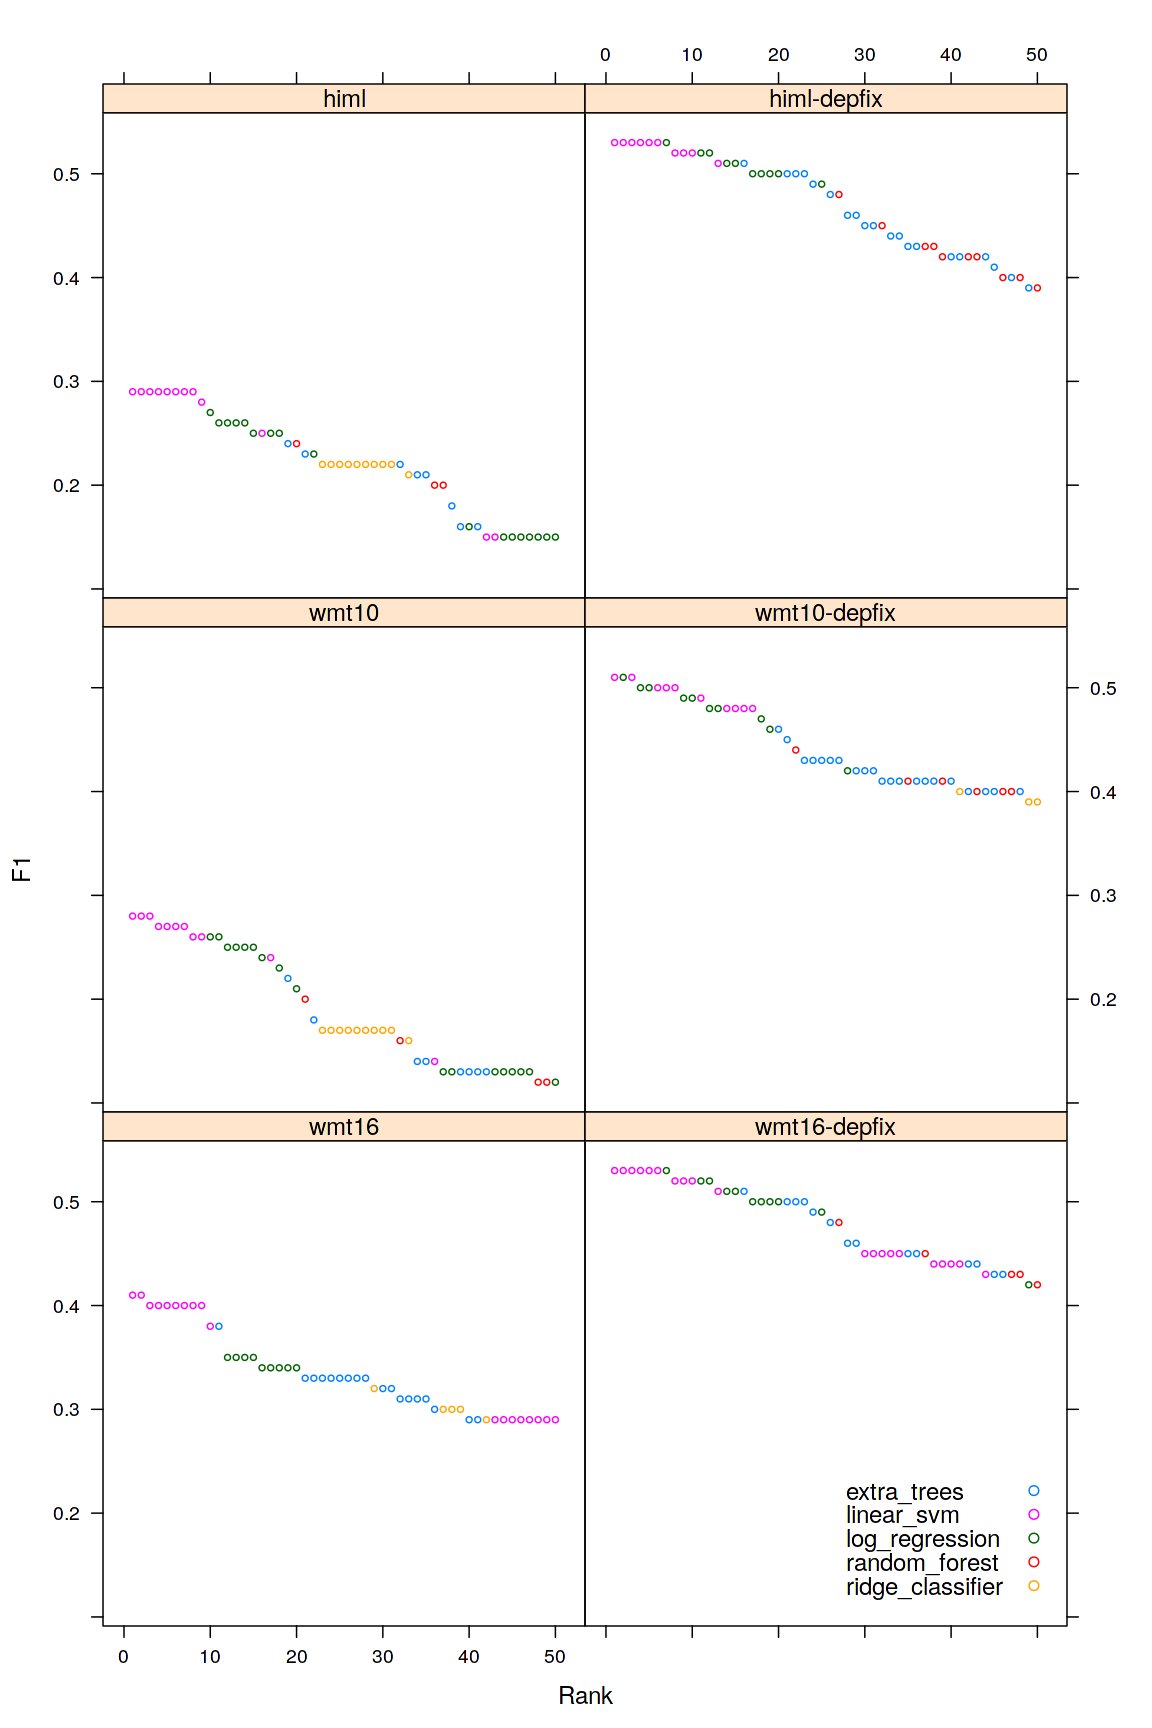
\includegraphics[scale=0.7]{wf-class}
  \caption{
    Overview of the classifier performance (error detection).
We have tried several variations of the hyperparameters
for each classifier. The classifiers are ordered from the best to the worst. Only top 50 results
are shown for each dataset.
}
  \label{wf-draft}
\end{figure}

\subsection{Feature Selection}

During model comparison, we have compared the performance on two initial feature sets:
one that did not contain any information about the source sentence ($\sim$680 initial features)
and one with source sentence features ($\sim$1360 initial features). Before training,
the features with zero variance were removed, however, no other feature filtering has been
performed. We have noticed that the additional information provided by the source sentence features
significantly improves performance of the majority of the ML methods. Therefore, we have decided
to use this feature set for feature selection method comparison.

Having selected SVM, we tried out several methods for feature
selection and compared their influence on the classifier performance. During the comparison,
we used a SVM model with fixed hyperparameters. We have compared the following methods for
feature selection: KBest selection (with chi-squared scoring function), selection of the percentile
of the features (based on the ANOVA F-test),
selection based on lasso regularization and selection through models with feature importance
scoring (svm, random forest). As far as importance scoring goes, we compared different
model configurations and during features selection, only features with importance higher
than the mean of the feature importance distribution were selected.

The results of feature selection method comparison are shown in~\Fref{wf-sel}. We can see
that most of the time the feature selection performed by either ANOVA percentile selector or
SVM slightly improved the model performance. Therefore, we have decided to use these methods during
the model tuning.

\begin{figure}
\centering
  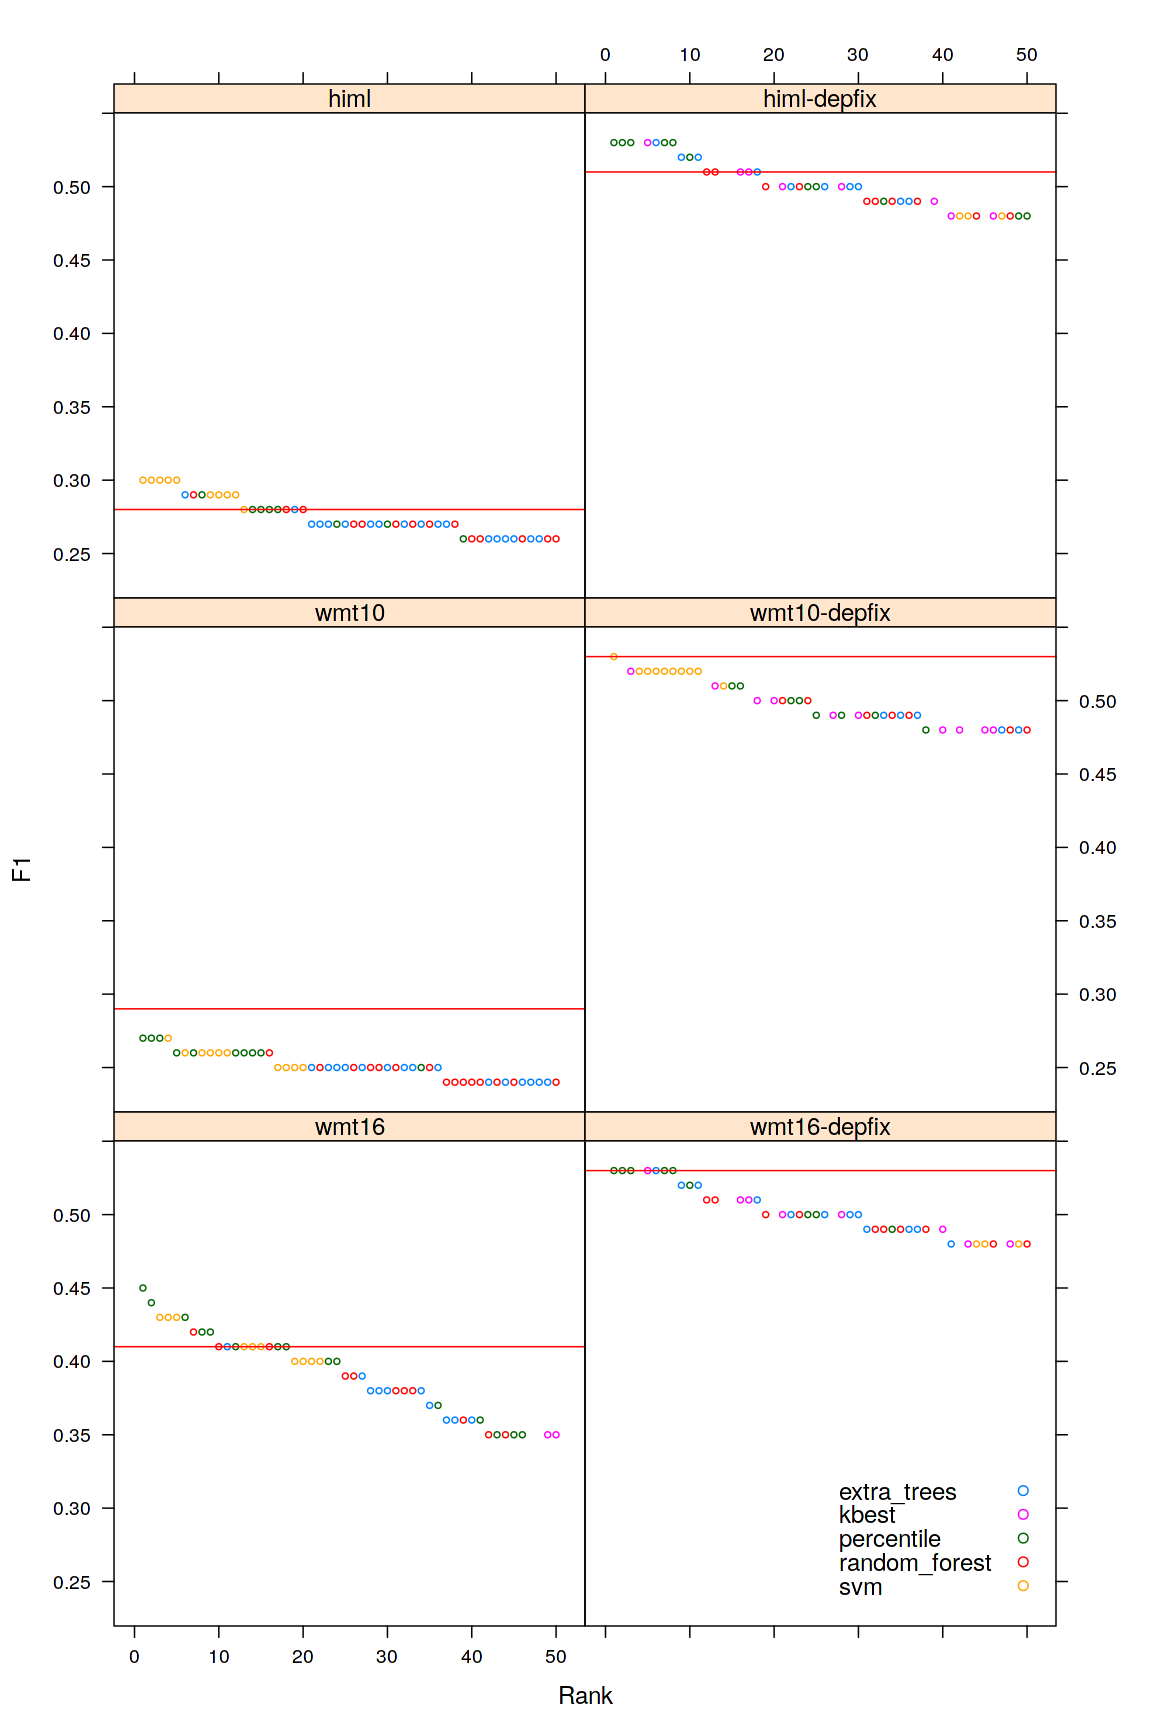
\includegraphics[scale=0.7]{wf-sel}
  \caption{
    Overview of the performance of the SVM with linear kernel when combined with various feature selection methods.
We have tried several variations of the hyperparameters
for each method. The horizontal line marks the best performance without
a feature selection method. The methods are ordered from the best to the worst. Only top 50 results
are shown for each dataset.
}
  \label{wf-sel}
\end{figure}

%TODO: feature representation - vectorized dicts, binary features???
% chceme to zminovat?

\subsection{Model Summary}

With the ML method and feature selection method chosen, we have proceeded to 
the development of the final model.
We have trained several different models, one for each presented dataset, instead of combining
the datasets and training one larger model. We have chosen this approach because it makes
it easier to exclude specific models if needed (e.g. during final evaluation) and in the
future, include additional models when more training data become available without the need
to retrain the whole error detection component. The use of multiple models for error detection
is described later in Chapter~\ref{chap:eval}.

We present the summary of the trained models in~\Tref{wf-summary}. We can see, that the models
trained on the Depfix data performed better than the ones trained on the original datasets. The overall
performance is still quite low, so there is still room for improvement. We think that introducing
additional features (e.g. information from the t-layer) or increasing the size of the training data
might help us improve these models in the future.

\begin{table*}[t]
\centering
\small

\begin{tabular}{lll|ccc}
Dataset  &  System  &  Ref  &  Precision  &  Recall  &  F1  \\
\hline
WMT10  &   CU-Bojar  &  REF  &  0.29  &  0.25  &  0.27  \\
HimL  &  Moses  &  PE  &  0.28  &  0.32  &  0.30  \\
WMT16  &  CU-Chimera  &  REF  &  0.40  &  0.44  &  0.42  \\
WMT10  &  CU-Bojar  &  Depfix  &  0.51  &  0.55  &  0.53  \\
HimL  &  Moses  &  Depfix  &  0.55  &  0.51  &  0.53  \\
WMT16  &  CU-Chimera  &  Depfix  &  0.50  &  0.52  &  0.51  \\
\end{tabular}
\caption{
    Final in-domain evaluation of the trained error detection models. The evaluation was performed
by a jack-knife one-vs-rest classification on each dataset. The \pojem{Origin} column indicates origin
of the reference data: poste-edited (PE), standard reference (REF) or created by Depfix.
}
\label{wf-summary}
\end{table*}


\section{Automatic Morphology Prediction}

The second classification task to predict correct morphological categories for
the words that were marked as incorrect. Because we are using the Interset representation
of the morphological features we have several possibilities, how to handle this task such
as:
\begin{enumerate}
    \item predict each category separately,
    \item concatenate the features and treat them as a single prediction target,
    \item use the methods that support multitask classification,
\end{enumerate}

With the first option, the biggest issue is determining the order in which the classifiers
should be aplied. Additionally we have to decide if we also want to include the current node's morphological features
into our model's feature set or use the newly predicted ones. The second approach eliminates this problem by predicting the
values simultaneously. However, this can quite easily expand the set of the predicted values,
which usually leads to increase in data sparsity. This can be a big problem as we have
already shown that the amount of data available for the post-editing task (mainly the post-edited
data) can be quite low. The third option combines the first two by training an estimator
which handles multiple joint classification tasks, one for each morphological category. The
Scikit-Learn toolkit provides several classifiers which support this option.

Before jumping straight into developing our classifier, it is important to examine what morphological
changes are made in our training data, how frequently they are made and how can they affect the resulting
surface form generation. For instance, we can predict new values of the \samp{punctype} category,
but it is very unlikely that it will affect the resulting wordform of any of the words
classified as incorrect, because this category is related strictly to punctuation. There are
of course less obvious examples and some categories, while being relevant in one target language
can be pointless in another.

For this reason, we have made a frequency analysis of the changes encountered
in our data, shown in~\Fref{iset-barplot}. We can see that most of the time, only the grammatical
case was modified (more than 50\% of the instances for the Depfix-based datasets and more than 40\% of the instances for
the normal datasets). Other changes were a lot less frequent (less than 10\% of the modified instances).
We have also checked, the amount of modifications made for individual general POS classes.
\Tref{changes-pos} summarizes the modification frequencies for each
POS class. As a conclusion, we have decided to focus on predicting the following categories: grammatical case, number, gender
and animateness. These categories are relevant to the majority of the changed words, therefore, changes made by
a classifer predicting these categories should be significant.

\begin{table*}[t]
\centering
\small

\begin{tabular}{lc}
POS  &  Frequency  \\
\hline
noun    &   38\%  \\
adj     &   16\%  \\
adp     &   10\%  \\
verb    &   9\%  \\
adv     &   9\%  \\
\end{tabular}
\caption{
    Part-of-speech (POS) frequencies of the changed words.
}
\label{changes-pos}
\end{table*}


\subsection{Machine Learning Method Comparison}

We have decided to train four different types of model: one predicting case only (C), one predicting case and number (CN),
 one predicting case, number and gender (CNG) and one predicting case, number, gender and animateness (CNGA).
We have used same datasets as in the previous task, however, this
time we have extracted only feature vectors of the instances that were marked as incorrect in our training data. Since
our predictors classify only the incorrect instances, training them on the whole dataset would only create
unnecesary bias. On the other hand, this has made the training sets quite small (containing only a few hundreds of examples
at most). The summary of the training data is in~\Tref{cats-training-sum}. We have decided to train a separate classifier
for each dataset instead of combining the data together, because we can simply combine the models instead (e.g. via majority
vote, best prediction etc.). This allows us to evaluate a combined model on a test set of our choice simply by leaving
out the model which was trained on that specific test set.

\begin{table*}[t]
\centering
\small

\begin{tabular}{lll|c}
Dataset  &  System  &  Origin  &  \hash{} training instances  \\
\hline
WMT10  &  CU-Bojar  &  REF  &  645  \\
HimL  &   Moses  &  PE  & 338  \\
WMT16  &  CU-Chimera  &  REF  &  722  \\
WMT10  &  CU-Bojar  &  Depfix  &  210  \\
HimL  &  Moses  &  Depfix  &  72  \\
WMT16  &  CU-Chimare  &  Depfix  &  99  \\
\end{tabular}
\caption{
    Summary of the size of the training data extracted from each dataset.
	\pojem{Origin} column indicates origin
	of the reference data: poste-edited (PE), standard reference (REF) or created by Depfix.
}
\label{cats-training-sum}
\end{table*}

Again, we had to decide which ML method should we use for this task. 
We have examined similar set of classifiers with similar
hyperparameters as in the error classification task to get a rough idea about their capabilities.
We have considered using the F-measure again, however, due to the nature of the training data (all
instances are classified), the model accuracy metric seemed more informative.
A rough comparison was made with the case classifier only.
Adding additional targets to the classifiers naturally lowers their overall accuracy,
however, their performance have been similar with respect to each other
The results are shown in~\Fref{cats-draft}. We can see, that even without any sophisticated parameter
tuning or feature filtering, the classifiers perform quite well. We can also notice that in most of the cases, the ensemble
methods (mainly extremely randomized trees) performed slightly better than the rest of the examined ML methods. Therefore, we have decided
to pick this method for further experiments.

\begin{figure}
\centering
  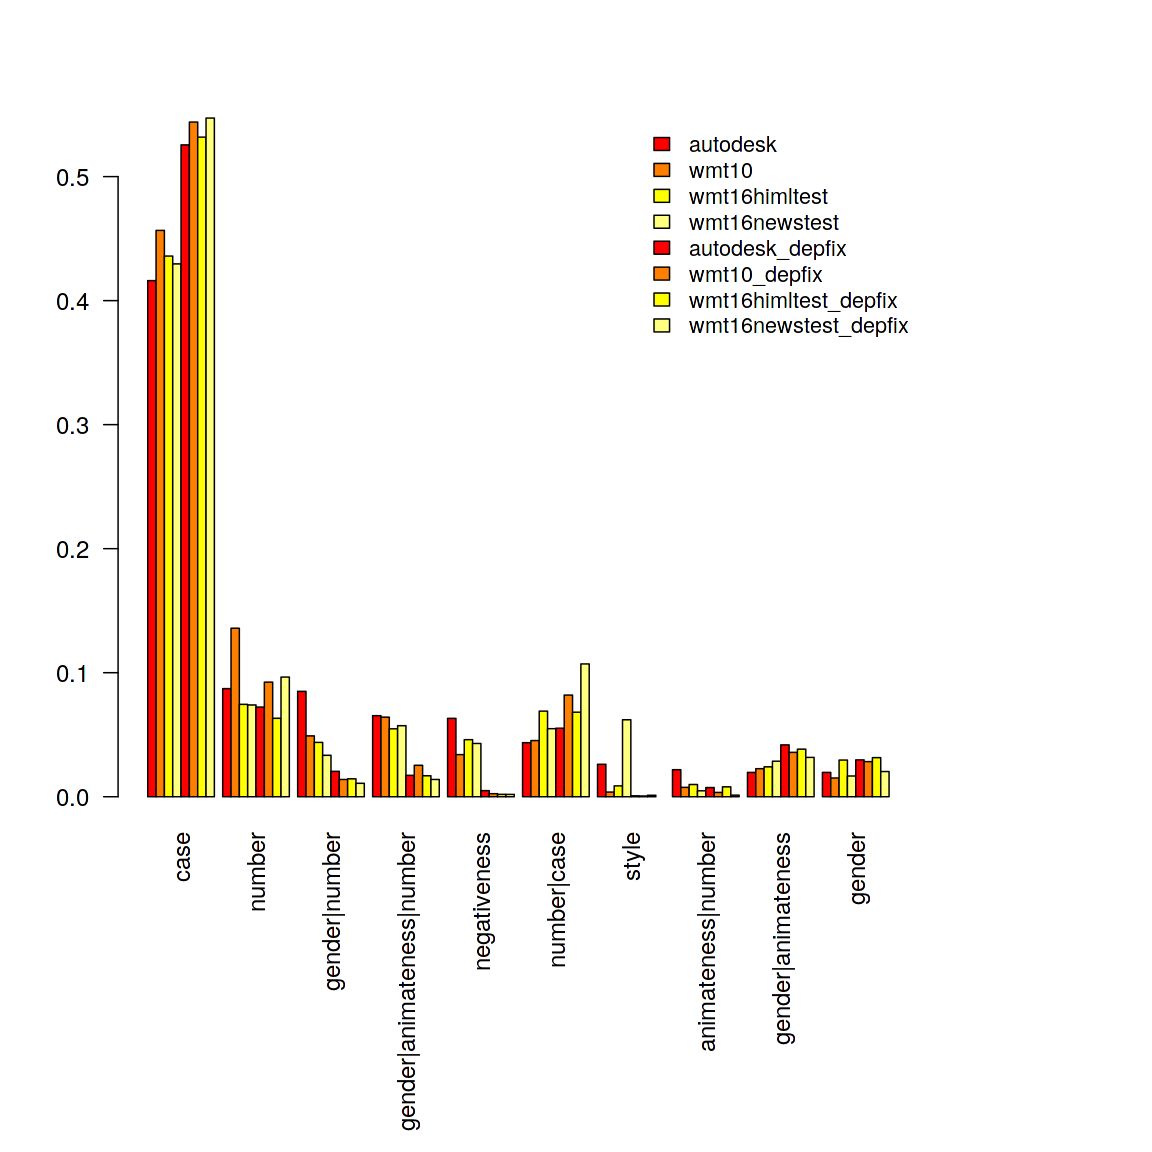
\includegraphics[scale=0.7]{iset}
  \caption{
    Frequency of the most changed Interset categories, grouped by a datasets. Categories containing
    "\textbar" symbol (e.g. gender\textbar{}number) represent changes made simultaneously.
}
  \label{iset-barplot}
\end{figure}

% with source
\begin{figure}
\centering
  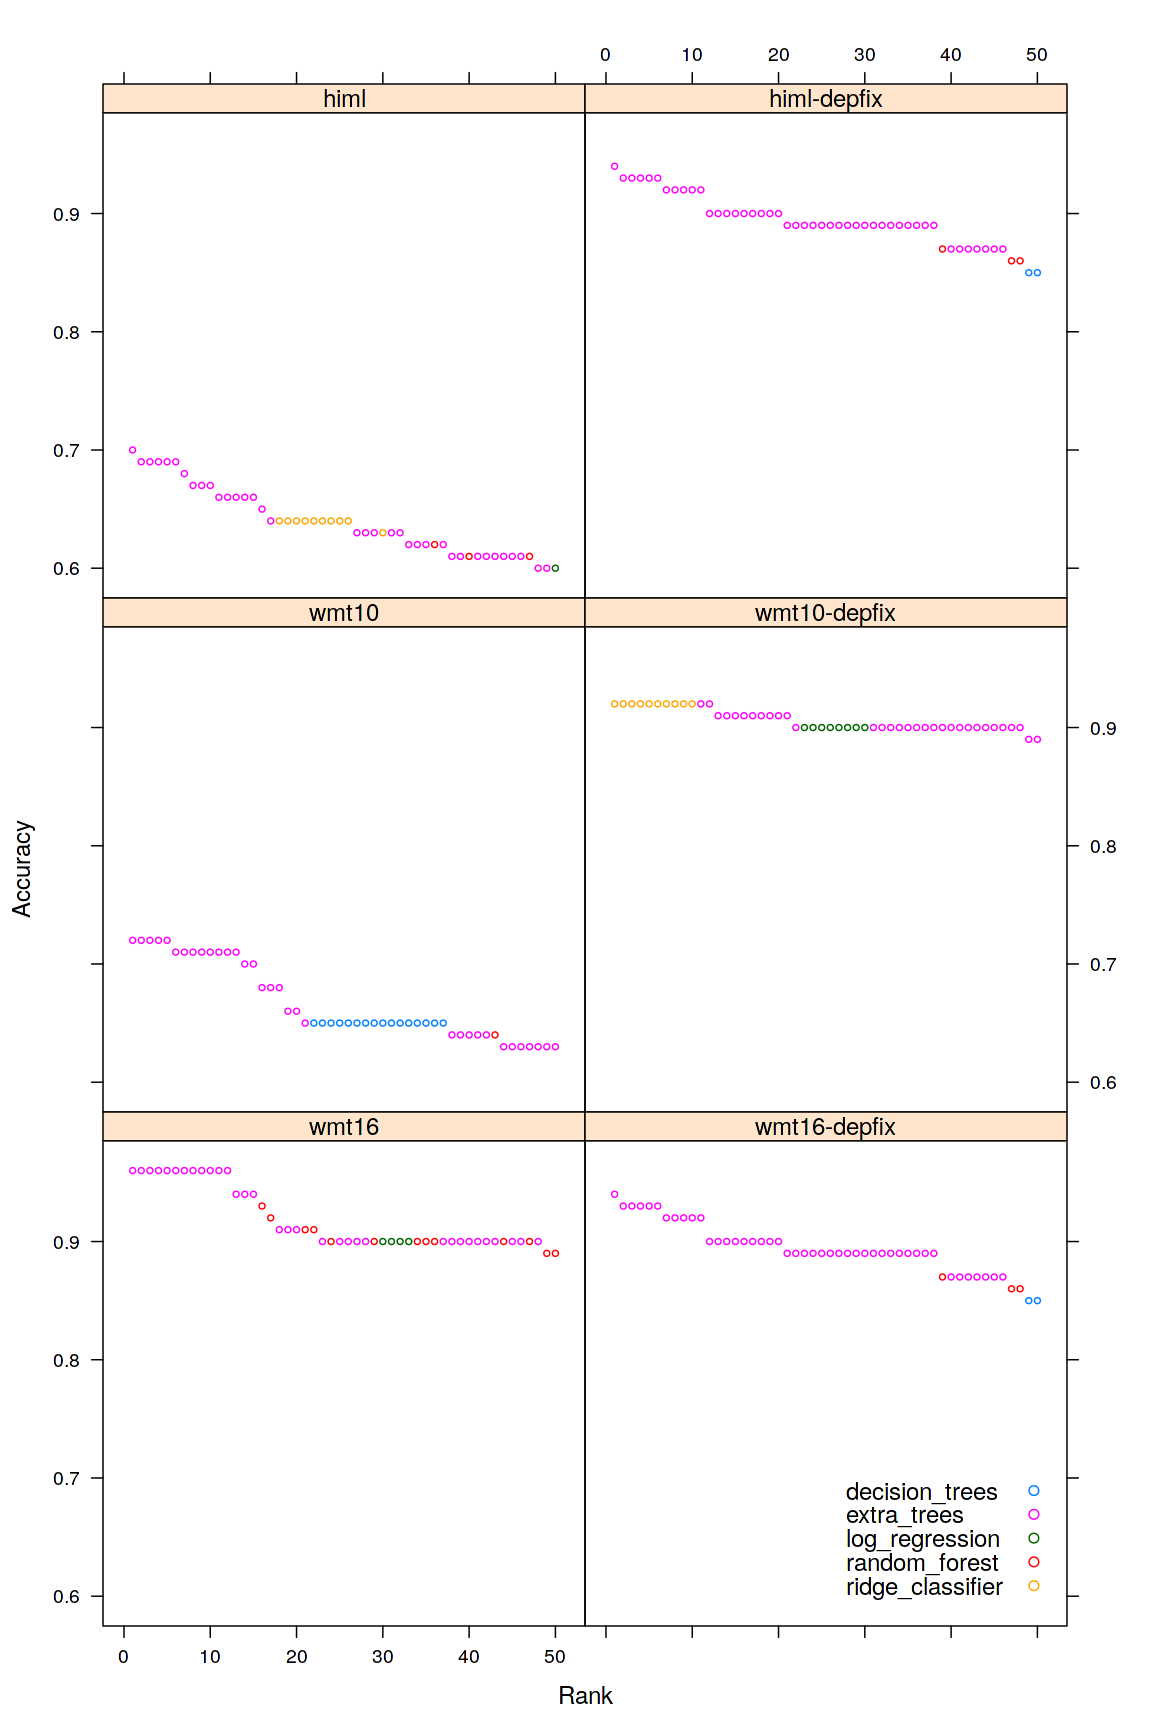
\includegraphics[scale=0.7]{cats-class}
  \caption{
    Overview of the classifier performance (category prediction).
We have tried several variations of the hyperparameters
for each classifier. The classifiers are ordered from the best to the worst. Only top 50 results
are shown for each dataset.
}
  \label{cats-draft}
\end{figure}

\subsection{Feature Selection}

We have decided to perform additional feature selection with models trained on the standard HimL dataset
and WMT10 dataset because there is still a reasonable room for an improvement. Again, we have tried two initial feature
sets, one using the source side features and one without them. We have not noticed any significant difference in performance
between models trained on these two initial feature sets so we decided to use the larger one and leave
the feature selection to the separate model. Additionally, due probably to the nature of the classifier, we have noticed
another slight improvement by adding the \pojem{source lemma} (both of the aligned node and its parent) feature, so we have also
included them to the initial features.\footnote{We have not included the \pojem{MT lemma} feature, because we wanted to
try using models trained on Czech for German post-editing and this feature is too language-specific for that purpose.}

We have compared several methods of feature selection: KBest selection
(with chi-squared scoring function), selection based on lasso regularization and selection through
models (svm, random forest). Again, we have done a rough comparison of these methods by trying out
several hyperparameter configurations. We tested them on a model with a fixed parameters. The result summary
is in~\Fref{cats-sel}. We can see that regarding HimL dataset, the feature selection did not have
any positive influence on the resulting model. On the other hand, we have decided to use the SVM-based
feature selection for the WMT10 dataset model training.

\begin{figure}
\centering
  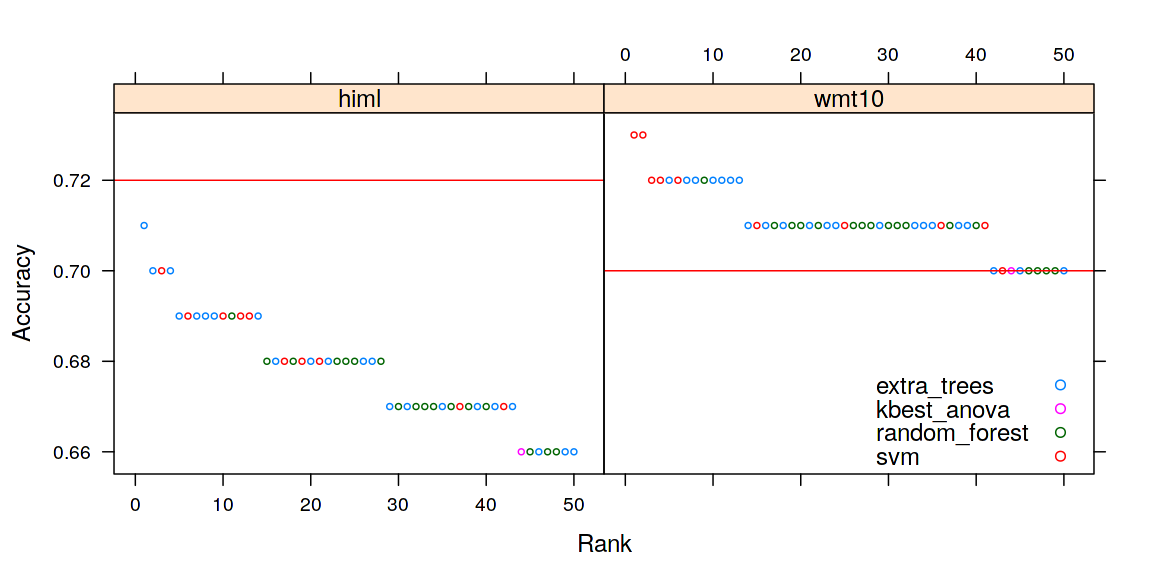
\includegraphics[scale=0.7]{cat-sel}
  \caption{
    Overview of the random forest performance when combined with various feature selection methods.
The methods are ordered from the best to the worst. The horizontal line marks the best performance without
a feature selection method. Only top 50 results are shown for each dataset.
}
  \label{cats-sel}
\end{figure}

%\subsection{Multitask models}
%todo???

\subsection{Model Summary}

In the end, we have trained six different models, one for the each dataset presented in the rough comparison.
Aside from the case clasiffier, we have also compared performance of the chosen multitask classifiers:
the case-number (CN), the case-number-gender (CNG) and the case-number-gender-animateness (CNGA)
classifier. These classifiers were trained using the same ML methods, each one was tuned separately.
The summary of the final in-domain performance is in~\Tref{cats-summary}.

We can see that by including additional target for the multitask classification the accuracy of the trained
model becomes naturally lower. However, we must take into account that we have only classified the predicted
values as correct or incorrect and we have not distinguished partially correct predictions. Brief overview
of the categories predicted by the CNGA classifer has shown us that usually a predictor misclassifies only
one or two of the target categories. Another thing to keep in mind is the fact, that even though the predicted
categories might not be equal to the gold standard, the generated surface form might still match the reference form
due to the morphological ambiguities of the language. For these reasons, we decided to use all these models during the system evaluation.

%Surprisingly, accuracy of the multitask models trained on WMT16 dataset dropped significantly when training a
%more complex classifier, underperforming even the baseline predictor. It is possible that the chosen ML
%method is not suitable for this dataset, even though it is performing well with the simple case classifier.

\begin{table*}[t]
\centering
\small

\resizebox{0.98\textwidth}{!}{
\begin{tabular}{lll|cccc}
Dataset  &  System  &  Origin  &  Case (Base)  &  CN (Base)  & CNG (Base)  &  CNGA (Base)  \\
\hline
WMT10  &  CU-Bojar  &  REF  &  73\% (35\%)  &  53\% (14\%)  &  40\% (7\%)  &  37\% (7\%)  \\
HimL  &  Moses  &  PE  &  72\% (34\%)  &  50\% (11\%)  & 41\% (5\%)  &  41\% (4\%)  \\
WMT16  &  CU-Chimera  &  REF  &  95\% (50\%)  &  45\% (21\%)  &  34\% (10\%)  &  32\% (10\%)  \\
WMT10  &  CU-Bojar  &  Depfix  &  92\% (45\%)  &  83\% (22\%)  &  69\% (19\%)  &  69\% (19\%)  \\
HimL  &  Moses  &  Depfix  &  92\% (47\%)  &  78\% (26\%)  &  73\% (23\%)  &  71\% (23\%)  \\
WMT16  &  CU-Chimera  &  Depfix  &  93\% (54\%)  &  64\% (16\%)  &  56\% (11\%)  &  53\% (9\%)  \\
\end{tabular}
}
\caption{
    Final in-domain model accuracy evaluation of the trained models. The evaluation was performed
by jack-knife one-vs-rest classification of the each dataset. Performance of the baseline (Base)
classifier is presented for comparison.
\pojem{Origin} column indicates origin
of the reference data: poste-edited (PE), standard reference (REF) or created by Depfix.
}
\label{cats-summary}
\end{table*}


%\todo{tohle az do final evaluace?}
%Since the domains of the datasets differ to a various degree, we have decided to combine the models trained
%on the different datasets, however, we do not combine different types of classifier. This combined model
%compares result of each separate classifier (with the prediction probability) and picks the most probable choice.


\chapter{System evaluation}
\label{chap:eval}

In this chapter, we will present the results of the MLFix system evaluation.
We will describe the datasets we have used during the evaluation and the different
configurations of MLFix we have compared. Furthemore we will present the evaluation
of the individual MLFix components.
We will also present a comparison with the Depfix
system. We have performed both automatic and manual evaluation.

\section{Automatic evaluation}

During automatic evaluation, we have used mainly BLEU\cite{papineni:2002} translation quality metric. However, we have also
measured Translation Edit Rate\cite{Snover06astudy} (TER) since it measures the amount of editing that is required by a human
to change the system output to match the reference translation. Even though the BLEU is widely used standard metric
used for SMT evaluation, we think that TER might be quite suitable for the evaluation too mainly because it indicates
how much aditional work is required to correct the SMT output.

We have evaluted MLFix on the following datasets: Autodesk, WMT10, WMT16, and HimL. All these datasets
were translated with the Chimera system. We have also measured the MLFix performance on the output of neural network
machine translation (NMT) system produced on the WMT16 dataset.

\todo{nejdriv komponenty, pak cely system s best configem?}
Since the domains of the datasets differ to a various degree, we have decided to combine the final models trained
on the different datasets. This combined model
compares result of each separate classifier (with the prediction probability) and picks the most probable choice.
We have used the combined model for the prediction of the new categories, for the error detection we have compared
the combined model with the best model


\subsection{Error detection evaluation}

\subsection{Category prediction evaluation}

\begin{table*}[t]
\centering
\small
\resizebox{0.9\textwidth}{!}{

\begin{tabular}{|l|l||c||c|c|c|c|c|c|}
\hline
Dataset  &  System  &  Oracle  &  Case  &  CN  & CNG  &  CNGA  & Comb  &  Comb-D  \\
\hline
\hline
Autodesk  &  NA  &  48.24  &  47.89  &  47.91  &  \bf{48.22}  &  48.21  &  47.90  &  47.90  \\
\hline
HimL  &  CU Chimera &  23.33  &  21.14  &  20.97  &  21.36  &  \bf{21.49}  &  21.03  &  21.08  \\
\hline
WMT10  &  CU Bojar  &  16.70  &  15.84  &  15.82  &  \bf{15.95}  &  \bf{15.95}  &  15.82  &  15.82  \\
\hline
\multirow{2}{*}{WMT16}  &  UEDIN NMT  &  27.31  &  26.43  &  26.48  &  26.47  &  \bf{26.50}  &  26.44  &  26.43  \\
&  CU Chimera  &  23.13  &  21.94  &  21.99  &  22.02  &  \bf{22.05}  &  22.02  &  21.94  \\
\hline
\hline
Autodek-D  &  NA  &  98.32  &  98.12  &  98.09  &  \bf{98.17}  &  98.16  &  98.08  &  98.10  \\
\hline
HimL-D  &  CU Chimera  &  96.05  &  95.23  &  95.04  &  95.41  &  \bf{95.42}  &  94.98  &  95.20  \\
\hline
WMT10-D  &  CU Bojar  &  95.72  &  95.03  &  94.99  &  \bf{95.10}  &  95.07  &  94.96  &  95.02  \\
\hline
WMT16-D  &  CU Chimera  &  97.51  &  97.22  &  97.23  &  97.26  &  \bf{97.27}  &  97.20  &  97.24  \\
\hline
\end{tabular}

}
\caption{
    Automatic evaluation of the morphological category prediction module. For comparison, evaluation of the
Oracle classifier is also provided. Datasets with the \pojem{-D} suffix have Depfix output in place of reference sentences.
}
\label{fixonly-summary}
\end{table*}

\section{Manual evaluation}

For manual evaluation, we have used the HimL dataset. We have used two independent annotators, both were presented with 
with a set of sentences randomly selected from the dataset.

A total of \todo{cislo} sentences were evaluated by the annotators. The results are shown in\todo{table}.
%okec

%okec k agreementu

\chapter{English-German}
\label{chap:german}

In this chapter we are going to describe changes we have made to an existing
English-Czech MLFix pipeline to be able to apply the system to the English-German
SMT outputs. We are going to summarize the data available for training the models
and evaluate the system in the system in a similar way we did with the English-Czech
pipeline.

\section{Processing pipeline modification}

As we have mentioned, we have focused on making the processing pipeline as independent
on the target language as possible. However, we still have to replace some of the tools
used for the Czech analysis to be able to correctly process German sentences.

Again, we have used the Treex framework as a backbone of the processing pipeline and
necessary 3rd party tools were implemented into the systems via wrappers.
After the sentences are read in parrallel, they are processed separately, English
following the same scenario as in the English-Czech pipeline.
German is again tokenized, this time by a set of regex rules inspired by Tiger corpus\cite{Brants2004}
with main focus on abbreviations, ordinal numbers and compounds connected by hyphens.

Next, lemmatization and POS tagging is performed by a Mate tools\footurl{http://www.ims.uni-stuttgart.de/forschung/ressourcen/werkzeuge/matetools.en.html}
toolkit. The tagger used CoNLL2009\cite{CoNLL-2009-ST} tagset. For tagging, we could have also
used the Stanford POS Tagger\footurl{http://nlp.stanford.edu/software/tagger.shtml}\cite{Toutanova:2000:EKS:1117794.1117802},
however, the tagset it uses contains only coarse tags without little morphological information.
To convert the CoNLL2009 tags to Interset, we use a decoder, which was already implemented at the
time of our research.

For the word alignment, we again use GIZA++. Similar to English-Czech, we produce one-to-one word alignment
with the intersetion symmetrization. We The alignment model has been trained on the European
Parliament Parallel corpus\cite{koehn2005epc}\footnote{http://www.statmt.org/europarl/} (Europarl)
containing nearly two million sentences. During the process of training data analysis we 
also create monolingual alignment between the MT output and the references sentences
in a similar way we did in the original pipeline.

The dependency structure for the MT output is again produced by projecting the English dependency
structures on the MT sentences. When processing the training data, we parse the reference sentences
by graph-based parser\cite{Bohnet:2010:VHA:1873781.1873792} implementation which is also a part of the
Mate tools toolkit. We stop the analysis at the a-layer, but again in the future, further analyzing
the sentences to the t-layer to gain additional features for extraction is desired.

We have reused the statistical component used in the English-Czech pipeline, because it was designed to be
language independent (with the exception of the statistical models). For wordform generation we have
the Flect morphological generation tool mentioned earlier. We have trained the generator on a small
fraction (around one hundred thousand sentences) of the Europarl corpus. The tool is trained on a set
of features based on a combination of lemma$+$Interset producing the inflected word.\todo{training data acc?}

\section{Data analysis}

We have been able to collect only a smaller variety of data for English-German compared to English-Czech
 mostly due to some datasets we mentioned earlier wer simply not available for this language pair. Still, we have been
available to gather following datasets: WMT16, HimL and Autodesk. Note that in case of Autodesk dataset,
the size of English-German is about three times bigger than the size of English-Czech (around 120k sentences).
For this reason, we have decided to include Autodesk dataset into our training data even though it covers
a limited domain.

When extracting the training instances for the statistical component we have followed same scenario
as before, using the same heuristic to identify \equo{incorrect} wordforms. We have also used the Oracle
classifier to gather information about possible improvements this heuristic can bring when applied to German.

We have also performed quick manual evaluation of the output produced by the Oracle classifier by a non-native
German speaker.
We have performed the evaluation on the WMT16 dataset this time because we have thought that medical domain of HimL dataset
would be too difficult for a non-native speaker to evaluate.
Due to limited
resources we have again used only a single annotator for this evaluation task. The evaluator, not being familiar
with the MLFix system, was presented set of instances containing the following: randomly shuffled MT output and Oracle output,
the source English sentence and the German reference translation. The results of the evaluation a shown in the table\todo{ref}
%okec

After the evaluation of our data extraction method we have analyzed the extracted instances and compared them
to the information we have gathered during Czech data analysis. The~\Fref{} shows the frequency of the changed Interset
categories.
%okec

We

%\todo{avail data?}
\todo{rozbory ala task\_descr?}
%\todo{oracle eval (human)}
\todo{changes - iset}
\todo{changes - pos}


\chapter*{Conclusion}
\addcontentsline{toc}{chapter}{Conclusion}


%%% Bibliography
%\include{bibliography}
\bibliographystyle{plainnat}
%\bibliographystyle{obo-bst}
\phantomsection
\addcontentsline{toc}{chapter}{Literature}
\bibliography{bib-varis}

%%% Figures used in the thesis (consider if this is needed)
\listoffigures

%%% Tables used in the thesis (consider if this is needed)
%%% In mathematical theses, it could be better to move the list of tables to the beginning of the thesis.
\listoftables

\appendix

%%% Abbreviations used in the thesis, if any, including their explanation
%%% In mathematical theses, it could be better to move the list of abbreviations to the beginning of the thesis.
%\chapwithtoc{List of Abbreviations}

%%% Attachments to the master thesis, if any. Each attachment must be
%%% referred to at least once from the text of the thesis. Attachments
%%% are numbered.
%%%
%%% The printed version should preferably contain attachments, which can be
%%% read (additional tables and charts, supplementary text, examples of
%%% program output, etc.). The electronic version is more suited for attachments
%%% which will likely be used in an electronic form rather than read (program
%%% source code, data files, interactive charts, etc.). Electronic attachments
%%% should be uploaded to SIS and optionally also included in the thesis on a~CD/DVD.
%\chapwithtoc{Attachments}
\chapter{MLFix scenarios}
\label{chap:scenario}

In this attachement we list both Czech and German scenarios we used for Depfix processing
pipeline. The scenarios are generated by the %\code{Treex::Scen::MLFix::} blocks, at the beginning
of the scenario there is a commented Treex command which generated the scenario. The scenarios
are listed in the order they are applied to the input. Note that the Czech and German blocks
are called only in their respective scenario.

\section{English-Czech}

\subsection{Analysis on m-layer}

\lstset{basicstyle=\ttfamily,breaklines=true}
\begin{lstlisting}

# Source (English)
# treex -d Scen::MLFix::Analysis_1 language=en iset_driver="en::penn"
Util::SetGlobal language=en selector=
Util::Eval zone='$zone->remove_tree("a") if $zone->has_tree("a");'
W2A::EN::Tokenize
W2A::EN::NormalizeForms
W2A::EN::FixTokenization
W2A::EN::TagMorphoDiTa lemmatize=0
W2A::EN::FixTags
W2A::EN::Lemmatize
A2A::ConvertTags input_driver=en::penn

# treex -d Scen::MLFix::NER language=en model=ner-eng-ie.crf-3-all2008.ser.gz
Util::SetGlobal language=en
A2N::EN::StanfordNamedEntities model=ner-eng-ie.crf-3-all2008.ser.gz
A2N::EN::DistinguishPersonalNames


# Target (Czech)
# treex -d Scen::MLFix::Analysis_1 language=cs tagger=morphodita iset_driver="cs::pdt"
Util::SetGlobal language=cs selector=
Util::Eval zone='$zone->remove_tree("a") if $zone->has_tree("a");'
W2A::CS::Tokenize
W2A::CS::TagMorphoDiTa lemmatize=1
W2A::CS::FixMorphoErrors
W2A::CS::FixGuessedLemmas
A2A::ConvertTags input_driver=cs::pdt
A2N::CS::SimpleRuleNER

# Reference (Czech)
# treex -d Scen::MLFix::Analysis_1 language=cs selector=ref tagger=morphodita iset_driver="cs::pdt"
Util::SetGlobal language=cs selector=ref
Util::Eval zone='$zone->remove_tree("a") if $zone->has_tree("a");'
W2A::CS::Tokenize
W2A::CS::TagMorphoDiTa lemmatize=1
W2A::CS::FixMorphoErrors
W2A::CS::FixGuessedLemmas
A2A::ConvertTags input_driver=cs::pdt
A2N::CS::SimpleRuleNER

\end{lstlisting}

\subsection{Alignment}

\begin{lstlisting}

# English-Czech
# treex -d Scen::MLFix::RunMGiza from_language=cs to_language=en model=cs-en
Align::A::AlignMGiza dir_or_sym=intersection selector= from_language=cs to_language=en model_from_share=cs-en tmp_dir=/mnt/h/tmp cpu_cores=1
Align::AddMissingLinks layer=a selector= language=cs target_language=en alignment_type=intersection
Align::ReverseAlignment language=cs selector=

# Reference
Align::A::MonolingualGreedy selector=T language=cs to_selector=ref

\end{lstlisting}

\subsection{Analysis on a-layer}

\begin{lstlisting}

# Source (English)
# treex -d Scen::MLFix::Analysis_2 language=en parser=mst
Util::SetGlobal language=en selector=
W2A::EN::ParseMST
W2A::EN::SetIsMemberFromDeprel
W2A::EN::RehangConllToPdtStyle
W2A::EN::FixNominalGroups
W2A::EN::FixIsMember
W2A::EN::FixAtree
W2A::EN::FixMultiwordPrepAndConj
W2A::EN::FixDicendiVerbs
W2A::EN::SetAfunAuxCPCoord
W2A::EN::SetAfun


# Target (Czech)
# treex -d Scen::MLFix::Analysis_2 language=cs src_language=en parser=
Util::SetGlobal language=cs selector=
A2A::ProjectTreeThroughAlignment language=en to_language=cs to_selector=

# Reference (Czech)
# treex -d Scen::MLFix::Analysis_2 language=cs selector=ref
Util::SetGlobal language=cs selector=ref
W2A::CS::ParseMSTAdapted
W2A::CS::FixAtreeAfterMcD
W2A::CS::FixIsMember
W2A::CS::FixPrepositionalCase
W2A::CS::FixReflexiveTantum
W2A::CS::FixReflexivePronouns

\end{lstlisting}

\subsection{Fixing}

\begin{lstlisting}

# Preparation
# treex -d Scen::MLFix::FixPrepare src_language=en tgt_language=cs
Util::Eval language=cs selector=T zone='$zone->remove_tree("a") if $zone->has_tree("a");'
Util::Eval language=cs selector=FIXLOG zone='$zone->set_sentence("");'
A2A::CopyAtree source_language=cs language=cs selector=T align=1
Align::AlignForward language=cs selector=T overwrite=0 preserve_type=0

# Fixing
# treex -d Scen::MLFix::Fix "mark_method=scikit-learn "fix_method=scikit-learn" "language=cs" "selector=" "mark_config_file=XXX" "fix_config_file=XXX" "iset_driver=cs::pdt"
MLFix::MarkByScikitLearn language=cs selector= config_file=XXX
MLFix::CS::ScikitLearn language=cs selector= config_file=XXX iset_driver=cs::pdt

\end{lstlisting}

\subsection{Detokenization}

\begin{lstlisting}

# treex -d Scen::MLFix::WriteSentences language=cs
Util::SetGlobal language=cs selector=
A2W::Detokenize
A2W::CS::DetokenizeUsingRules
A2W::CS::DetokenizeDashes
Util::Eval zone='print $zone->sentence . "\n";'

\end{lstlisting}

\section{English-German}

\subsection{Analysis on m-layer}

\begin{lstlisting}

# Source (English)
# treex -d Scen::MLFix::Analysis_1 language=en iset_driver="en::penn"
Util::SetGlobal language=en selector=
Util::Eval zone='$zone->remove_tree("a") if $zone->has_tree("a");'
W2A::EN::Tokenize
W2A::EN::NormalizeForms
W2A::EN::FixTokenization
W2A::EN::TagMorphoDiTa lemmatize=0
W2A::EN::FixTags
W2A::EN::Lemmatize
A2A::ConvertTags input_driver=en::penn

# treex -d Scen::MLFix::NER language=en model=ner-eng-ie.crf-3-all2008.ser.gz
Util::SetGlobal language=en
A2N::EN::StanfordNamedEntities model=ner-eng-ie.crf-3-all2008.ser.gz
A2N::EN::DistinguishPersonalNames


# Target (Czech)
# treex -d Scen::MLFix::Analysis_1 language=de tagger=mate iset_driver="de::conll2009"
Util::SetGlobal language=de selector=
Util::Eval zone='$zone->remove_tree("a") if $zone->has_tree("a");'
W2A::DE::Tokenize
W2A::DE::LemmatizeMate
W2A::DE::ParseMate lemmatize=0
A2A::DE::CoNLL2Iset

# Reference (Czech)
# treex -d Scen::MLFix::Analysis_1 language=de selector=ref tagger=mate iset_driver="de::conll2009"
Util::SetGlobal language=de selector=ref
Util::Eval zone='$zone->remove_tree("a") if $zone->has_tree("a");'
W2A::DE::Tokenize
W2A::DE::LemmatizeMate
W2A::DE::ParseMate lemmatize=0
A2A::DE::CoNLL2Iset

\end{lstlisting}

\subsection{Alignment}

\begin{lstlisting}

# English-German
# treex -d Scen::MLFix::RunMGiza from_language=de to_language=en model=de-en
Align::A::AlignMGiza dir_or_sym=intersection selector= from_language=de to_language=en model_from_share=de-en tmp_dir=/mnt/h/tmp cpu_cores=1
Align::AddMissingLinks layer=a selector= language=de target_language=en alignment_type=intersection
Align::ReverseAlignment language=de selector=

# Reference
# Align::A::MonolingualGreedy selector= language=de to_selector=ref

\end{lstlisting}

\subsection{Analysis on a-layer}

\begin{lstlisting}

# Source (English)
# treex -d Scen::MLFix::Analysis_2 language=en parser=mst
Util::SetGlobal language=en selector=
W2A::EN::ParseMST
W2A::EN::SetIsMemberFromDeprel
W2A::EN::RehangConllToPdtStyle
W2A::EN::FixNominalGroups
W2A::EN::FixIsMember
W2A::EN::FixAtree
W2A::EN::FixMultiwordPrepAndConj
W2A::EN::FixDicendiVerbs
W2A::EN::SetAfunAuxCPCoord
W2A::EN::SetAfun


# Target (German)
# treex -d Scen::MLFix::Analysis_2 language=de src_language=en parser=
Util::SetGlobal language=de selector=
A2A::ProjectTreeThroughAlignment language=en to_language=de to_selector=

# Reference (German)
# treex -d Scen::MLFix::Analysis_2 language=de selector=ref
Util::SetGlobal language=de selector=ref
W2A::DE::ParseMate
A2A::DE::CoNLL2Iset

\end{lstlisting}

\subsection{Fixing}

\begin{lstlisting}

# Preparation
# treex -d Scen::MLFix::FixPrepare src_language=en tgt_language=de
Util::Eval language=de selector=T zone='$zone->remove_tree("a") if $zone->has_tree("a");'
Util::Eval language=de selector=FIXLOG zone=$zone->set_sentence("");
A2A::CopyAtree source_language=de language=de selector=T align=1
Align::AlignForward language=de selector=T overwrite=0 preserve_type=0

# Fixing
# treex -d Scen::MLFix::Fix mark_method=scikit-learn fix_method=scikit-learn language=de selector= mark_config_file=XXX fix_config_file=XXX iset_driver=de::conll2009
MLFix::MarkByScikitLearn language=de selector= config_file=XXX
MLFix::DE::ScikitLearn language=de selector= config_file=XXX iset_driver=de::conll2009

\end{lstlisting}

\subsection{Detokenization}

\begin{lstlisting}

# treex -d Scen::MLFix::WriteSentences language=de
Util::SetGlobal language=de selector=
A2W::Detokenize
Util::Eval zone='print $zone->sentence . "\n";'

\end{lstlisting}



\openright
\end{document}
